%e WORDY word checks
%--------------------------------------------------------------------------------
% - weasel
% - weak
% - puffy
% - ditto
%--------------------------------------------------------------------------------

\section{Introduction}
\label{sec:introduction}
% intro structuring basing on style from https://explorationsofstyle.com/2013/01/22/introductions/
%Intro short:
% - recent developments of of A.I. and machine learnin
% - most research problems applied to image recognition, translation and in the RL space to games and robotics.
% - global warming, lots of problems
% - reinvent the energy grid, lots of changes to the structure
%   - very difficult to construct such a highly complex, globally spanning, must-never-fail system
% - combine the two

%Intro long
% - energy grids of the future background research (PTac)
%     - key components of such an intelligent agent (prediction, actions --> supervised learning and \ac{RL} )
% - research in supervised learning and \ac{RL} has seen huge improvements in recent years, thanks to neural network
% - agents/brokers in the field of PTac haven't been seeing much of these improvements
% - also an issue of "adopting what has been learned by previous agents (transfer learning issues)"
% -
% -

% Global warming is a key challenge of the near and medium future. Without proper action, entire continents will see
%
% Global warming, if not combated, will change the face of the planet. Billions will be impacted, entire coastlines will
% be changed and cities all over the global will have to either be retrofitted to handle sub-sea level positioning or
% abandoned and relocated. (global warming report)
%
%
% One key component to avoid such disastrous effects is the reinvention of the energy systems of the world. While
% appliances on an individual level need to become ever more efficient, globally it is necessary to shift the
% transportation sector towards renewable energy sources.
% Solar and wind
% are required. But The future of energy is difficult (--> MISQ paper argumentation line)
%
% Smart grids need decentralized intelligence where appliance level evaluation of the grid status impacts how energy is
% consumed. When such intelligence shifting is happening towards the \emph{edge} of the grid, it can be intelligent to
% introduce intermediate broker entities that mediate between the two extremes, the end-consumers and the wholesale
% market.
%
% At the same time, current developments in AI and machine learning allow for highly sophisticated learning machines that
% can help manage complex tasks and systems. (citing some sexy AI papers)
%
% Bringing these two developments together, it is intuitive to apply some of the recently developed technologies of
% \ac{AI} research to solve the coordination issues of contemporary, frankly crude energy networks.

%-------------------------------------------------------------------------------
% Done v1, looking over it again at the end
%-------------------------------------------------------------------------------

In recent years, \ac{AI} research saw a steady rise in publications and overall interest in the field
\citep{arulkumaran2017brief, russell2016artificial}.
It has been discussed as a key future challenge for nation states and companies alike
\citep{mozur_markoff_2017, faznetchina_2018}. Researchers have produced a large corpus of research focusing on visual
data learning such as image recognition, audio and text based language recognition and robotics. In the field of
\ac{RL}, recent breakthroughs were achieved by applying it to robotics as well as common game challenges like solving Atari games or
playing Go
\citep{arulkumaran2017brief}.

There are other important problem fields that can also benefit from these technologies, one of them being global energy markets.
These are expected to shift radically in the upcoming decades, adapting to new problems related to global warming,
distributed and alternative energy sources, lack of intelligently coordinated systems, cybersecurity  and electric vehicles \cite[p.10ff.]{mitei2011}. New problem solving techniques are required to solve such \emph{wicked problems}, because
they depend on numerous elements such as economic, social, political and technical factors.
\citep{ketter2015competitive}.

On a local scale, but much more prominently in day-to-day life, machines need to deliver their performance with minimal
energy requirements. Cars, fridges, water heating appliances, dishwashers and entertainment systems alike have all shown
improvements in their efficiency and this has become a key component of a customer's purchasing choice.  Similarly,
large distributed IT systems as well as building management systems are adapted to make more efficient use of the energy
they consume \citep{Orgerie:2014:STI:2597757.2532637}. A key driver in this field is
the usage of intelligent systems that adapt to changing environments and demands \citep{DePaola:2014:IMS:2620784.2611779}.

On a macro scale, the problem is just as complex, albeit less salient.  Electricity grids were conventionally not built
to contain \emph{energy buffers}. Electricity always needed to be produced to match demand. This is expected to change
over the coming years due to an increasing number of electric vehicles and smart appliances. Such systems can serve as
buffers
by offering their storage capacity to the grid, which is needed because decentralized
solar energy production changes the demand curve of macro-level energy supply. As an example, California is currently
facing an
oversupply of energy during sunny summer days and undersupply during peak demand hours that intersect with low levels of
solar energy production. This puts previously unseen stress on the grid systems which were constructed to deliver steady amounts
of energy from a few sources to many consumers instead of having many small producers distributed throughout the system.
Furthermore, large conventional power plants struggle to adapt quickly to change in demand patterns
\citep{roberts_2016}.

\ac{PowerTAC}, a competitive simulation of future energy markets, attempts to solve the planning dilemma of such
complex systems. It allows researchers to experiment with numerous scenarios and participant designs. By adapting system
parameters, robust system designs are developed to incentivize participants to align with the overall
interests. The interaction of a variety of market participants using different technologies to automatically generate
profit is explored in a competitive game environment. Researchers are invited to participate in this simulation by
supplying usage models for appliances and developing \emph{brokers} that participate in the game.  Brokers trade energy,
offer contracts and coordinate storage capacities within their own customer network as well as with the overall market.
The simulation offers opportunities for several fields of research: game design, energy demand forecasting,
intelligent contract design, commodity trading and general simulation and software design
\citep{ketter2015competitive, ketter2018powertac}.

The competition has been organized for several years and brokers can be developed by anyone. This means that some
broker developers have years of experience while others have not participated in a single competition. Previous researchers have
identified the problem as a \ac{POMDP}, a common model of \ac{RL} literature \citep{tactexurieli2016mdp}. Deep neural network
architectures have proven to be successful in solving games in a variety of instances. It is intuitive to
attempt to apply such architectures to the problems posed by the \ac{PowerTAC} simulation. Unfortunately, most of the
implementations are only available in Python \citep{baselines, plappert2016kerasrl, schaarschmidt2017tensorforce}  and
\ac{PowerTAC} is almost exclusively based on Java. An extension of the current communication protocols to other
languages may increase the reach of the simulation and motivate newcomers to join the competition with
their Python-based neural network architectures.

Finally, a sub field of \ac{RL} research has identified a problem in the transfer of knowledge from previously trained
networks to newly developed iterations. Because neural networks are mostly black boxes to researchers
\citep{yosinski2015understanding}, it is difficult to extract knowledge and to transfer this to another architecture. The
learned weights of a neural network can not be easily transferred between models, especially when architectures fundamentally
differ in their hyperparameters. The field of transfer learning has shown new approaches for solving this problem.
Agents with access to previously developed models may pass their observations to the \emph{teacher agent} and initially
attempt to align their decisions to those that their teacher would do \citep{schmitt2018kickstarting}. High level
problem solving agents may be trained by first training several small narrow focus agent networks on sub problems and
then applying transfer learning to transfer the knowledge from the narrow focus agents to the generic high level
agent \citep{parisotto2015actor}. For problems where a reward function is difficult to construct, \emph{inverse
reinforcement learning} can be used to train an agent to behave similar to an observable expert. The policy function of
the agent shows good performance despite lacking a specific reward function \citep{NG2004Apprentice}.

In summary, neural networks are an interesting technology to solve complex problems and energy markets stand to benefit from
their usage. To ensure beneficial results, \ac{PowerTAC} simulates complex energy markets before implementing them in the real
world. \ac{PowerTAC} focuses on brokers as intermediaries between end consumers and wholesale markets to reduce
complexity and to decentralize which also aids resilience. To allow current and future teams competing in the \ac{PowerTAC}
competition to easily deploy neural network technologies and to allow new brokers in the \ac{PowerTAC} competition to quickly
catch up to previously developed competitor brokers, it may be beneficial to extend the technology scope of the
competition and enable learning transfer methods and their underlying deep architectures for the problem scope of
\ac{PowerTAC}. Therefore, the research question for this work goes as follows:

\emph{Can deep reinforcement learning agents learn from actions of other agents in the \ac{PowerTAC} environment? If so,
    how? Can imitation allow for boosted performance of reinforcement learning algorithms within a competitive simulation
environment?}



\subsection{Methodology}
\label{sec:methodology}
To answer the questions, a lot of foundation work has to be done. First, the competition needs to be able to interface
with the technologies required by modern neural network frameworks. Then,  a problem mapping needs to occur to map the
\ac{PowerTAC} problems to a structure that frameworks and libraries can work with. Finally, current research methods for
learning transfer need to be applied to the \ac{PowerTAC} environment. Consequently, this work follows a practical
software development approach, and this document also serves as a documentation to accompany the implementation. The
practical part of the thesis consists of the concepts for integrating \ac{PowerTAC} and the libraries and tools of
modern \ac{RL} research, then implementing all the necessary components to bridge the gap. The implemented source code is
often tested with unit tests to ensure the correct functioning of the components. Once all components are
developed to connect the two areas, machine learning approaches need to be applied to create solutions for the demand
prediction problem and the wholesale trading problem.

This document is structured as follows: first, the literature of the fields of \ac{AI}, \ac{RL} and the \ac{PowerTAC}
competitive simulation for energy markets is reviewed. In the field of AI its sub fields of supervised learning and
unsupervised learning will be introduced. Here, the focus is placed on the area of neural networks and a way to let them
learn through Backpropagation. In the field of \ac{RL} the focus is on the \ac{MDP} framework.  Next follows an
introduction of the recent research concerning the use of neural networks in \ac{RL} settings to allow the so-called
\ac{DeepRL}. For \ac{PowerTAC}, its concepts and how agents (often called brokers in the context of \ac{PowerTAC}) make
decisions are analyzed, including an analysis of previous agents solution approaches. 

%After having introduced the basic research of \ac{AI} and \ac{RL}, I will summarize the state of research of Animal
%Cognition, which focuses on how animals and humans learn, act and remember in their environment. Since humans and
%animals are the only known form of intelligent life to us as of today, it is intuitive why exploring the exact workings
%of these examples might help in better understanding how to artificially create intelligence. It is also a basis of the
%thesis, as many animals show forms of social learning, concepts of teaching and learning through observation.

Following the theoretical background, an analysis of a number of observation based learning approaches is performed.
Three alternative approaches for learning from other agents or historical data are discussed conceptually.

In the practical part, the main technologies used are briefly explained. Then follows a summary of the implementation
of two important decision areas, wholesale trading and demand predicting. Both implementations demonstrate
the ability to use current research results from the neural network and \ac{RL} research community to apply them to the
\ac{PowerTAC} problem set.

Finally, a conclusion is drawn together with a discussion of the limits and weaknesses as well as recommended further research.


%This chapter will introduce the two underlying research fields, \ac{AI} and the \ac{PowerTAC} simulation. The broad
%field of \ac{AI} will be separated into three sections: an introduction to the fields of \ac{AI}, neural networks and \ac{RL}.
%\ac{PowerTAC} will be discussed by introducing it, comparing it to similar work and analyzing its
%components and some dominant past broker implementations.

\section{Artificial Intelligence}%
\label{sec:artificial_intelligence}

%-------------------------------------------------------------------------------
% done unless professor adds notes
%-------------------------------------------------------------------------------

The field of \ac{AI} is both old and yet quiet contemporary.
Right with the advent of computers around the middle of the 20th century, research has started to aim for artificial
intelligence. Generally, defining \ac{AI} in a single sentence is hard. \citet{russell2016artificial} structures
historical definitions along two dimensions: the grade of how \emph{human} \texttt{XOR} \emph{rationl} a system
\emph{thinks} \texttt{XOR} \emph{behaves}. These four directions are all pursued by researchers. In
this thesis, the goal of \emph{behaving rationally} is the most appropriate sub field of research in the larger field of
\ac{AI}.

Today, some 70 years later, \ac{AI} is again extensively discussed by both researchers and main-stream media
\citep[p.24ff.]{russell2016artificial, arulkumaran2017brief}. The reasons for this are diverse but it can be argued that
the combination of easily available computing power through cloud computing and advances in the mathematical
underpinnings have allowed for fast-paced advances in recent years. Also, the currently popular neural network
architectures often require large amounts of data to learn which have lately been readily available for companies and
researchers through the adoption of online technologies by the majority of the population
\citep[p.27]{russell2016artificial}.

\subsection{Learning}
\label{sec:learning}

According to \citep{russell2016artificial}, learning agents are those that \emph{improve their performance on future
tasks after making observations about the world} \cite[p.693]{russell2016artificial}. Among living animals, learning
behavior is present in many species. The general goal of \ac{AI} research is to imitate these
skills to dynamically adapt
to unforeseen environments. To create a learning algorithm doesn't require the creator to anticipate every
potential variant of an environment that the learning agent is confronted with while still creating a successfully
acting agent. Cognitive Sciences define learning as the change of state due to experiences and often limit the
recognition of learning to some externally observable behavior \cite[p.96f.]{cognition1999}. This applies to all known
species and the same definition can easily be applied to a learning artificial agent. A learning agent that doesn't
change its behavior is not helpful and an agent that doesn't change its internal state can hardly have learned
something.

In \ac{AI} research, a \emph{loss function} is commonly used as a measure of learning progress. Loss functions describe
the difference between the actual utility of the right actions versus the results of the agents learned actions. The
exact loss function might be a mean squared error function or an absolute loss depending on the learning algorithm that
is used or whether the researcher intends to emphasize large deviations from the target \cite[p.710]{russell2016artificial}.

Computational learning theory looks at different problems of learning: how to learn through a large number of
examples, the effects of learning when the agent already knows something, how to learn without examples, how to learn
through feedback from the environment and how to learn if the origin of the feedback is not deterministic
\citep{russell2016artificial}. In this work, two of those problems are of special interest: the ability to learn from
previously labeled examples and the ability to learn through feedback from the environment. The former is called
supervised learning and the latter is referred to as \acl{RL}. To understand the difference, it is also important to
understand algorithms that don't have access to labels of existing data, yet are still able to derive value from the
information. These belong to the class of unsupervised learning. Although this class is not heavily relied upon in the
later implementation of the agent , it is crucial for tasks in machine learning such as data exploration or anomaly
recognition.

The following sections will describe both supervised learning and unsupervised learning and section~\ref{sec:neural_networks} will introduce
an architecture that can be used as the learning function in these learning problems. Finally,
Section~\ref{sec:Backpropagation} will explain how exactly neural networks learn.

\subsubsection{Supervised Learning}


%-------------------------------------------------------------------------------
% done unless professor adds notes
%-------------------------------------------------------------------------------

As noted above, supervised learning uses labeled examples to learn to recognize future examples that might be of the
same kind but not identical \cite[p.695]{russell2016artificial}. Common examples of this form of learning include object recognition in images or
time-series prediction. One of the most known examples to date is the Imagenet classification algorithm by
\citep{krizhevsky2012imagenet} which was one of the first neural network based algorithms to break a classification high-score
on a popular image classification database. The goal is to correctly classify images according to a set of defined
labels. If a picture of a dog is read by the neural network, it needs to be able to classify the fact that a dog is in the
picture. In trading environments it can be helpful to be able to predict future patterns based on current and previous
observations. In the space of machinery, learning to recognize sensor data that indicates faulty parts can be used to
avoid down-time of machines through preemptive replacement during scheduled service intervals \citep{rudin2012machine}. In the online marketing
industry, recognizing user interests to send appropriate ads benefits just as well from the approach as do spam filters
that recognize ads and filter them out again \citep{domingos2012few}.

The general problem of supervised learning is as follows:

\begin{enumerate}
    \item Generation of a \emph{training set} that holds a set of input-output pairs \\ $(x_1,y_1),(x_2,y_2),\ldots$
    \item Training of algorithm against training set
    \item Verification of results against a previously unseen \emph{test set}
\end{enumerate}

If $y$ can be any of a given set of answers, the problem is a \emph{classification} problem and if the problem requires the
prediction of a potentially infinite number of alternatives (e.g.\ a real number between 1 and 10), it's a
\emph{regression} problem. The outputs $y_n$, or labels, are created based on an underlying true function $f$ which the
algorithm tries to learn or approximate through a function $h$, the hypothesis. The space of hypotheses is infinitely
large and the general principle, called \emph{Ockhams razor} , is that simpler hypotheses with equal performance as more complex
ones are to be preferred. By deciding up-front about the decision space (e.g.\ all linear functions) the best hypothesis
might not be able to perfectly match the underlying true function $f$. On the other hand a hypothesis chosen from such
an expressive hypotheses space may generalize well and it is easier to understand and implement.

The tradeoff described above is a key factor when deciding on the \emph{right} function to use to solve a supervised
learning problem. A linear regression model is easier to understand than complex convoluted functions and neural
networks have
often been described as hard to interpret as it is not clear \emph{what} they learn. Systems such as decision trees,
which make many sequential decisions about features of the input in question to arrive at a classification, are easy to
interpret and might be more appropriate when not only the performance of the system is important but also the
inner workings of it \citep[p.696ff.]{russell2016artificial}.


\subsubsection{Unsupervised Learning}
%-------------------------------------------------------------------------------
% done unless professor adds notes
%-------------------------------------------------------------------------------
Unsupervised learning suffers from one key difference: the set of data that is used to learn from lacks labels or
classifications. In other words, there are no examples to indicate what it is that needs to be
learned. Common examples of unsupervised learning are \emph{clustering} or \emph{principal components analysis}. The
overall goal of unsupervised learning is not to predict but to learn information about the underlying distributions and
reasons as to why the values have been measured in a certain way. Unsupervised learning is also used during pre-processing
data for supervised learning problems to improve the later results of the regression or classification problems
\cite[p.373f.]{james2013introduction}.
Additional features can be constructed from results of unsupervised learning such as distances to cluster centers. These
additional features may then also be fed to the learning algorithm. Doing so is risky, as it may introduce
implicit biases of the data analyst.

\subsection{Neural Networks}%
\label{sec:neural_networks}


%-------------------------------------------------------------------------------
% done unless professor adds notes
%-------------------------------------------------------------------------------
\begin{figure}[b]
    \centering
    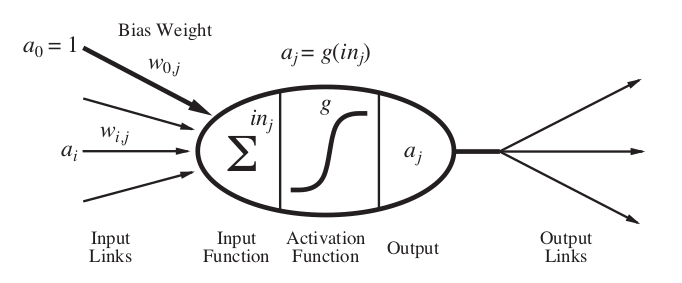
\includegraphics[width=0.8\linewidth]{img/perceptron.png}
    \caption{Model of the perceptron, taken from \citep{russell2016artificial}.}
    \label{fig:perceptron}
\end{figure}

Neural networks are a technology that is used to approach problems from both supervised learning and unsupervised learning problems. The original
concept can be dated  as far back as 1943 \cite[p.727]{russell2016artificial} and the mathematical description of a
neuron is a linear combination of many input variables $a_i$ and their weights $w_i$. If the linear combination of the
input variables exceeds a threshold, defined by an activation function $g$, the neuron activates or \emph{fires}. When
the activation function $a$ results in a binary value, it is called a \emph{perceptron}. Real value outputs are possible
through a different, non binary activation function. These are often logistic functions and the resulting unit is
sometimes called a sigmoid perceptron \cite[p.729]{russell2016artificial}. A visual model of this unit
is given in Figure~\ref{fig:perceptron}.


A neural network  is a collection of such neuron components, often layered. The properties of the neurons as well
as the overall network properties are called \emph{hyperparameters} and describe the overall architecture of the neural network.

A common architecture is the \emph{feed-forward network} which holds several layers of sets of neurons. Each set has no
connection within itself but its activation output is fed into the next layers neurons. It is a directed
acyclic graph. Other than the weights, this network has no internal state and can not hold information about
the input in some form of memory. An alternative is a \emph{\acl {RNN} } which includes loops and can
hold state. The former network is often used for image classification problems while the latter is used for
time-series analysis and natural language processing.

When looking at neural networks one important decision is the number of layers. In fact, the history of neural networks has shown
three key phases of progress, the first phase which included simple single-layer networks, the second which included one
\emph{hidden layer} and the third phase, today, which uses networks that benefit from several hidden layers. A hidden
layer is a number of neurons between the input layer and the output layer. This allows the network to generate complex
input-output relationships. Such a multi-layer network is conceptualized in Figure~\ref{fig:multilayernn}. Each layer
$h^n$ feeds into the next until the output layer is reached \citep[p.729ff.]{russell2016artificial}.

\begin{figure}[]
    \centering
    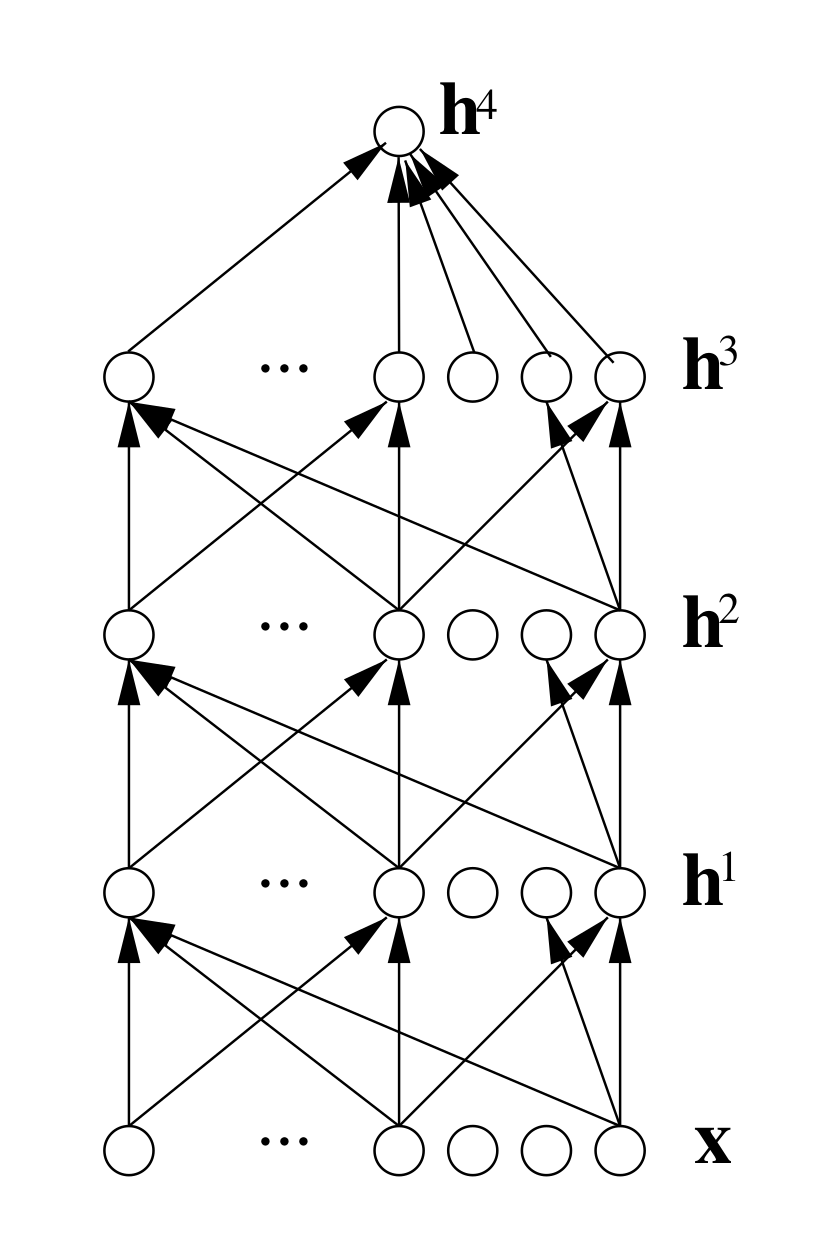
\includegraphics[width=0.3\linewidth]{img/multilayer_nn.png}
    \caption{Multi-layer neural network from \citep{bengio2009learning} }
    \label{fig:multilayernn}
\end{figure}

Neural networks can represent complex non-linear and discontinuous functions
\cite[p.732]{russell2016artificial} even with small numbers of layers or neurons. Such \emph{deep} networks however long
suffered from a large issue: it was unclear how to train them, i.e.\ how to make them learn. The next section describes
a solution to this problem.

\subsubsection{Learning Neural Networks and Backpropagation}
\label{sec:Backpropagation}


%-------------------------------------------------------------------------------
% done unless professor adds notes
%-------------------------------------------------------------------------------


The previous sections have described learning in respect to the goal of the learning process and the input data that is
used to learn from. This section explains the forms of learning and focuses on one widely used form called \emph{backpropagation}.

When looking at neural networks while remembering the earlier definition of learning, it becomes clear that there are many
ways a neural network can change its state. It could:

\begin{enumerate}
    \item develop new connections
    \item remove existing connections
    \item change the connecting weights
    \item change the threshold values of the activation functions
    \item change its input function
    \item develop new neurons
    \item remove existing neurons \cite[p.60]{kriesel2007brief}
\end{enumerate}

\noindent Of these many actions, changing the weights is the most common way to let a neural network learn. This is because many
of the other changes in its state can be performed by a specific way of changing the weights. Removing connections is
equivalent to setting the weight of the connection to 0 and forbidding further adaption afterwards. Equally, adding new
connections is the same as setting a weight of 0 to something that is not 0. Changing the threshold values can also be
achieved by modeling them as weights. Changing the input function is uncommon. The addition and removal of neurons
(i.e.\ the growing or shrinking of the network itself) is a popular field of research but will not be discussed further
\cite[p.60]{kriesel2007brief}.

Learning by changing the weights covers a wide range of possible adaptions to the network structure. When
looking at a single (sigmoid) perceptron, the changing of the weights of its input values is the same process as that of the
concept of gradient descent algorithms. Because the activation function is most often \emph{soft} to ensure
differentiability and because a hard threshold creates a non-continuous function, the process of fitting the weights to
minimize loss is called logistic regression \cite[p.729f.]{russell2016artificial}. For a detailed explanation of the gradient
descent approach, refer to the works of \citet{russell2016artificial} as well as
\citet{Goodfellow-et-al-2016}.



%logistic regression + gradient descent on a unit based view

The above described concept of learning from labeled examples is intuitive for single-layer neural network. The output can be
directly compared to the labels provided by the training set and logistic regression can be applied to correct the weights of
the network to reduce the loss. It becomes problematic though, when several layers are inserted between the input and
the output. The weights of the hidden layers are not included in the labeled examples. This is where the concept of
backpropagation becomes useful. For Figure~\ref{fig:multilayernn}, any error of the weights of the neurons in
layer $h^1$ influence the values of the output of layer $h^2$ and $h^3$ (in the case of fully connected layer).
However, for any additive loss function (such as $L_2$) the error is simply the sum of the gradients of the losses of
the outputs \cite[p.733f.]{russell2016artificial}. For a given $L_2$ loss it is

\begin{equation}
    \frac{\partial}{\partial w} Loss(w) =  \frac{\partial}{\partial w} \vert y-h_w(x) \vert ^2 = \frac{\partial}{\partial w} \sum_k{(y_k - a_k)^2} =  \sum_k{\frac{\partial}{\partial w}(y_k - a_k)^2}
    \label{equ:errorssum}
\end{equation}

\noindent where $w$ is the weight of the target neuron, $y$ the target value and $k$ the index of the nodes in the
output layer \cite[p.733f.]{russell2016artificial}. Even though this does not
solve the issue that the training set doesn't include the expected values for the hidden layers, this is solved by
back-propagating the error values through the network. Each previous hidden neuron is considered to be partially
responsible for a downstream error in relation to its weight in the target neuron.

\subsubsection{Recurrent Neural Networks}%
\label{sec:recurrent_neural_networks}

As was already noted in the previous chapter, neural networks can be both acyclic and cyclic graphs. The
\emph{vanilla} neural network is usually considered to be an acyclic feed-forward network, as it has no internal state
and it is more suited to describe the concepts of how the networks operate. Especially in translation and text to speech
applications, \ac{RNN} are popular as they are able to act on previously seen information in a sequence of
data. Generally they are suitable for many applications where the data has time-dependent embedding
\cite[p.373]{Goodfellow-et-al-2016}.

A \ac{RNN} computes its output based on the weights $w_i$, commonly noted as $\theta$, it's current input
$x^t$ and it's previous hidden units internal states $h^{t-1}$.

\begin{equation}
    h^t = f(h^{t-1}, x^t, \theta)
\end{equation}

\noindent The network generally learns to use $h^t$ to encode previously seen aspects relevant to the current task, although this
is inherently lossy as the previous number of inputs (i.e.\ $\mid t-1\mid$) is arbitrary. Figure~\ref{fig:rnn_concept}
shows this concept.

\begin{figure}[]
    \centering
    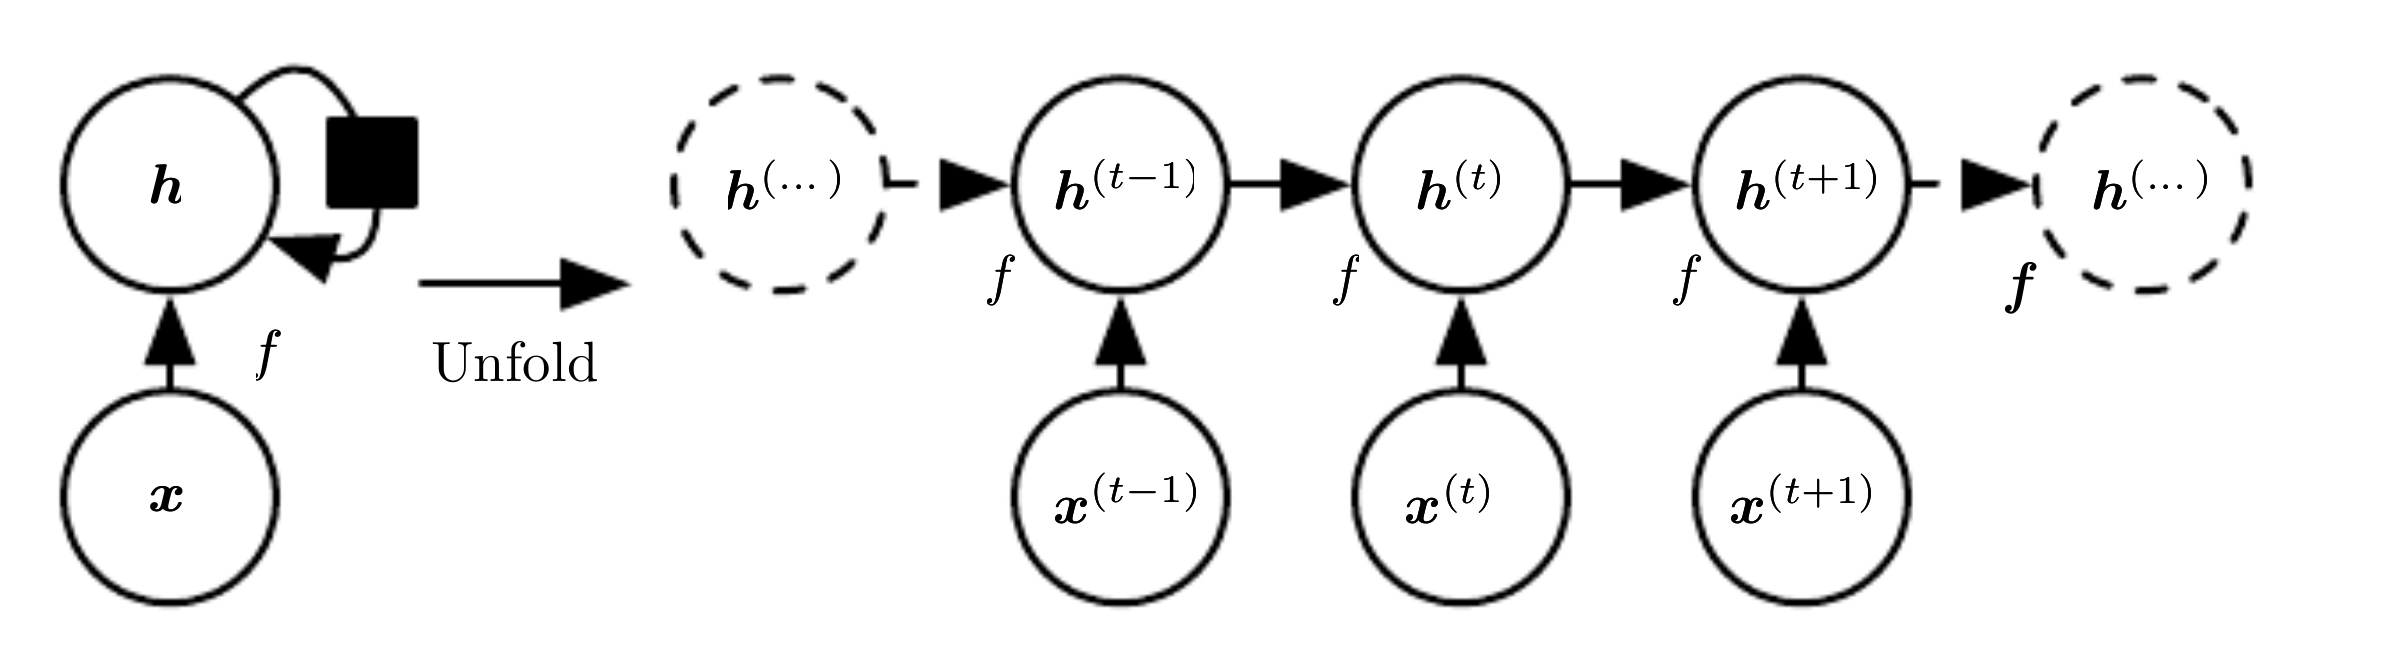
\includegraphics[width=0.8\linewidth]{img/rnn_concept.png}
    \caption[Recurrent Neural Network conceptualized]{. \emph{Left}: circuit diagram where the black square represents a
        1 time slot delay. \emph{Right:} The same network unfolded where each node represents a particular time instance.
    Taken from \citet{Goodfellow-et-al-2016}.}
    \label{fig:rnn_concept}
\end{figure}

The network structure has two benefits: firstly, it allows for arbitrary sequence length, as the network size is
dependent on the time slot specific input and not on the number of previous time slots. Secondly, the same network with
the same weights (or in mathematical terms the same transition function $f$) can be used during each time slot. This
means: when a \ac{RNN} is fed a sequence of data, the weights will stay the same throughout the sequence. They can be
updated after the entire sequence has been processed.

Such recurrent systems, while theoretically able to hold information across inputs, suffer from an issue called the
\emph{vanishing gradient problem}. A network that sequentially processes 20 samples is not easily capable to hold useful
information within its state from the early beginning to then act upon it later in the sequence. This is a common
problem for translation: sentences often have structures where the first word influences the meaning of the final one.
The network processes each word at a time, diluting the information that is representing the first word because it
is covered with noise from the other (potentially irrelevant) words. \citet{Hochreiter:1997:LSM:1246443.1246450}
developed the \ac{LSTM} model to solve this problem. Each unit in the network is actually a group of gates that act in
harmony to store information in a recurrent cell. \ac{LSTM} implementations differ between libraries, but they generally
follow the same core concepts. Modern TensorFlow-based implementations offer \ac{GPU} acceleration which significantly
increases performance and allows for distributed calculation.


\subsection{Reinforcement Learning}
\label{sub:rl}

The previous chapters have introduced concepts of supervised learning, neural networks, backpropagation and recurrent
neural networks for time-embedded
learning tasks. \ac{RL} can be described as an intersection between supervised and unsupervised learning concepts and
Deep \ac{RL} is the usage of neural networks, especially those with many layers, to perform \ac{RL}.

On the one hand \ac{RL}  does not require large amounts of labeled data to enable successful systems which is
beneficial for areas where such data is either expensive to acquire or difficult to clearly label. On the other hand it
requires some form of feedback. Generally, \ac{RL} \emph{agents} use feedback received from an \emph{environment}.  The
general principle of \ac{RL} includes an agent and the environment where it performs actions. The function
that determines the action $a$  taken by the agent in a given state $s$ is called its policy, usually represented by
$\pi$.  The environment reacts to the actions of the agent by returning new states $s'$ which are evaluated and a
corresponding reward $r$ is given to the agent. The reward gives the agent information about how well it performed
\citep[p.830f.]{russell2016artificial}.

This section will first introduce the concepts of a \ac{MDP}, then introduce different concepts of \ac{RL} agents,
describe approaches to encourage exploration of its options and finally describe how neural networks can be used to create
state-of-the-art agents that can solve complex tasks. The majority of Section~\ref{sub:rl} is based on
chapters 17 and 21 of \citet[]{russell2016artificial} unless it is marked otherwise.

\subsubsection{Markovian Decision Processes}%
\label{ssub:markovian_decision_processes}

A common model describing the conceptual process of states and actions followed by new states and new actions of an
agent and its environment is called a \acf {MDP}. In fact, \ac{RL} is an approach to optimally solve \ac{MDP} problems.
A \ac{MDP} is usually defined by the following components:

\begin{itemize}
    \item $\mathcal{A}$: Finite set of allowed actions
    \item $\mathcal{S}$: Finite set of states
    \item $P(s' \mid s,a) \forall s \in \mathcal{S}, a \in \mathcal{A}$: Probability of transitioning from state
        $s$ to state $s'$ when action $a$ is taken
    \item $\gamma$: Discount factor for each time slot, discounting future rewards to allow for long-term and
        short-term focus
    \item $R(s)$: Reward function that defines the reward received for transitioning into state $s$
\end{itemize}

To solve an \ac{MDP}, an agent needs to be equipped with a policy $\pi$ that allows for corresponding actions to each
of the states. The type of policy can further be distinguished between \emph{stationary} and \emph{non-stationary}
policies. The former type refers to policies that recommend the same action for the same state independent of the
time step. The latter describes those policies trying to solve non-finite state spaces, where an
agent might act differently once time becomes scarce. However, infinite-horizon \ac{MDP} can also have
terminal states which conceptually mean that the process has ended.

A more complex form of \ac{MDP} is the \ac{POMDP} which involves agents basing their actions on a belief of the
current state. However, as the later practical application to \ac{PowerTAC} can be mapped to a \ac{MDP}
where the transition probability implicitly represents the partial observability \citep{tactexurieli2016mdp}, this will not be discussed.

\subsubsection{Bellman Equation}%
\label{ssub:bellman_equation}

The Bellman Equation offers a way to describe the utility of each state in an \ac{MDP}. For this, it defines the
utility of a state as the reward for the current state plus the sum of all future rewards discounted by $\gamma$.

\begin{equation}
    U(s) = R(s) + \gamma \max_{a\in\mathcal{A}(s)} \sum_{s'}{P(s' \mid s,a)U(s')}
\end{equation}

\noindent In the above equation, the \emph{max} operation selects the optimal action in regard to all possible actions. The
Bellman equation is explicitly targeting \emph{discrete} state spaces. If the state transition graph is a cyclic graph
the solution to the Bellman equation requires some equation system solving. That is because $U(s')$ may depend on $U(s)$
and the other way around. Further, the \emph{max} operator creates non linearity that quickly becomes intractable for
large state spaces. An iterative approach called \emph{Value Iteration} is considered a valid alternative.

%In a discrete action space this would be a selection over all possible actions, in a continuous action space it however
%can become more complex. neural network based \ac{RL} agents simply invoke their policy network to retrieve the action which
%the agent believes it the one with the highest utility \citep{mnih2013playing}.


%As an example, an agent active in the environment of playing Super Mario may receive rewards corresponding to the game
%score. It may perform all valid moves permitted by the game and the goal is to improve its score.

%To train an agent, the task is usually performed several times and the environment is reset after each iteration to
%allow for a new learning step.
%When thinking about such an agent, it becomes obvious that without some explicit incentive to explore new alternatives,
%it may be contempt with whatever success it achieves and then always perform the same action. To avoid this, the agent
%can either be forced to try new alternative actions (through forcing random actions in a certain percentage of cases) or
%through explicit rewards for random actions.


%There are several forms of learning to solve a \ac{MDP} using \ac{RL} but for the purpose of this thesis I will focus
%on explaining how policy search algorithms work. Their goal is to find a good policy $\pi$ given a certain state $s$.
%Alternatives to this approach are concepts that try to learn expected future reward for future possible states, for
%available actions and others.

\subsubsection{Value and Policy Iteration}%
\label{sub:policy_and_value_iteration}

Value Iteration uses the Bellman equation to iteratively converge towards a correct estimation of each states utility,
assuming both the transition function $P(s' \mid s,a) \forall s \in \mathcal{S}$ and the reward function $R(s)$ are
known to the agent.
In the algorithm, the utility of each state is updated based on the \emph{Bellman update} rule:
\begin{equation}
    U_{i+1}(s) \gets R(s) + \gamma \max_{a \in \mathcal{A}(s)} \sum_{s'}{P(s' \mid s,a) U_i(s')}
\end{equation}
This needs to be performed for \emph{each} state during \emph{each} iteration. It is clear how quickly this becomes
intractable when $\gamma$ is reasonably close to 1, meaning that also long-term rewards are taken into
consideration.

However, the agent doesn't care much about the values of various states. It cares about making the right
decisions, using the value of states as a basis for doing so. It is often observed that the policy $\pi$ converges far
sooner than the utility estimates $U(s)$. This is the basis for the \emph{Policy Iteration} approach which alternates
between:
\begin{enumerate}
    \item evaluating the current policy $\pi_i$ by calculating $U_i=U^{\pi_i}$, the value of each state if $\pi$ is
        executed and
    \item improving the policy using one-step look-ahead based on $U_i$
\end{enumerate}

\noindent This process stops when the policy is no longer showing any significant improvements in respect to its loss value. It is
generally also not necessary to always apply the above operations to \emph{every} state. Instead, state values and
policies can be updated only in respect to newly discovered knowledge regarding specific states or specific actions.
This is called \emph{asynchronous policy iteration}.

Both variants require the transition function and the reward function to be known to the agent. \ac{RL} research has
developed several methods that adapt the concepts of the two iteration algorithms for environments with the two unknown
functions. They are explained in the next sections.
%It allows for many interesting concepts to be used such as distributed learning, using multiple agents to explore an
%environment and learn from all their observations centrally, and

\subsubsection{Temporal Difference Learning}%
\label{sub:temporal_difference_learning}

When the underlying transition function is not known, but the agent has the ability to perform many trial runs in the
environment, an empirical approach can be adapted. Therefore, the agent performs a number of trials where it acts
according to a (fixed) policy and observes the rewards it receives. Each string of alternating actions and observations
is called a trial.
The update rule for the utility of each state is
\begin{equation}
    U^\pi(s) \gets U^\pi(s) + \alpha(R(s) + \gamma U^\pi(s') - U^\pi(s))
\end{equation}
where $\alpha$ is the learning rate and $U^\pi$ the utility under the execution of $\pi(s)$ in state $s$. This only
updates the utilities based on the observed transitions so if the unknown transition function sometimes leads to
extremely negative rewards through rare transitions, this is unlikely to be captured. However, with sufficiently many
trials, these rare probabilities will be adequately represented in the utilities for the states. A continuous reduction
of $\alpha$ leads to conversion on the correct value.

\subsubsection{Exploration}%
\label{sub:exploration}

The above learning approach has one weakness: it is only based on observed utilities. If $\pi$ follows the pattern of
always choosing the action that leads to the highest expected $U_{i+1}$, i.e.\
\begin{equation}
    \pi(s) = \max_{a \in \mathcal{A}(s)}P(s' \mid s, a)U(s')
\end{equation}
then it will never explore possible alternatives and will very quickly get stuck on a rigid action
pattern mapping each state to a resulting action. To avoid this, the concept of \emph{exploration} has been introduced.
There are many approaches to encourage exploration. The simplest way is to define a factor $\epsilon$ which defines the
probability of choosing a random action at each step.

A more advanced variant is to add a term to the loss function that corresponds to negative entropy of the policy $-\beta
H(\pi(a \mid s ))$ where $H$ measures the entropy of a series of actions. The encourages randomness in the policy but
it permits the policy function to determine how this randomness occurs \citep{schmitt2018kickstarting}. This
entropy based loss also automatically regulates itself: when the agent is not at all able to choose rewarding actions
it reduces its loss through high entropy choices, i.e.\ lots of exploration. Once the agent finds actions for certain
states that lead to high rewards, choosing other random actions negatively outweighs following the best action.
Therefore, it becomes less random and the entropy reduces. If $\beta$ is progressively lowered, the impact on the loss
is progressively lowered, allowing the agent to continuously improve its loss despite less exploration.
Another alternative is the positive weighting of actions in states that have not been tried yet, essentially giving such
actions an optimistic prior as if they promise higher rewards than the already explored regions. This is easy to
implement for small, discrete state and action spaces but more complex for continuous spaces.

% Q Learning and Deep-Q learning
% Policy Gradient


\subsubsection{Q Learning}%
\label{sub:q_learning}

Section~\ref{sub:policy_and_value_iteration} already described how to learn the values of states, given an
action. This action can also be derived from a policy function. When an agent wants to learn its policy
(i.e.\ learn what a good policy is), it becomes problematic if the transition function is not known. An alternative
model is called \emph{Q-Learning} which is a form of Temporal Difference Learning. It learns an action-utility value
instead of the state values. The relationship between the \emph{Q-Value} and the former value of a state is
\begin{equation}
    U(s) = \max_{a}Q(s,a)
\end{equation}
so the value of a state is that of the highest Q-Value. This approach is beneficial because it does not require a model
of how the world works, it therefore is called a \emph{model-free} method. The update rule for the Q-Values is
the Bellman equation with $U(s)$ and $U(s')$ replaced with $Q(s,a)$ and $Q(s',a')$ respectively.

The update rules for the Q-Value approach are related to the Temporal Difference Learning rules but include a $\max$
operator
\begin{equation}
    Q(s,a) \gets Q(s,a) + \alpha(R(s) + \gamma \max_{a'}Q(s', a') - Q(s,a))
\end{equation}
An alternative version is the reduction of the above equation by removing the $\max$ operator. This results in the
\emph{actual} action being considered instead of the one that the policy believes to be the best. Q-Learning is
\emph{off-policy} while the latter version, called \ac{SARSA}, is \emph{on-policy}. The distinction has a significant
consequence: while Q-Learning may be used to learn the Q-Values from recorded state-action pairs, \ac{SARSA} requires
the action taken to be derived from the current policy function.

\subsubsection{Policy Search and Policy Gradient Methods}%
\label{sub:policy_search_and_policy_gradient_methods}

These two approaches are possibly the simplest of the \ac{RL} algorithms. In its most basic form, policy search requires
the algorithm to start with an initial policy to then adapt it until no further gains can be made. While the
concept is simple, it may lead to significant performances, if the \emph{choices regarding what to change} are made
wisely. If the policy is just randomly changed, the results will be equally random. However, if the policy is changed depending
on a good interpretation of the environment's responses, this method can offer good performance without the need
to have a model of how the world works. Such an agent takes the current state $s$ as input and uses its policy to
determine an output action $a = \pi(s)$. The value of a policy is noted as $\rho(\theta)$.

For simplicity, actions from a policy are assumed to be continuous as the later application relies on
such actions and because the analysis of policy search algorithms becomes more complex in discrete action spaces. When
both the policy and the environment are deterministic and without noise, policy search algorithms are effective.
The agent can repeat actions in the equivalent states several times, adapting its policy parameters $\theta$ by small
values and determining the empirical gradient values, allowing the agent to perform hill-climbing in the policy
function. This will converge to a local optimum, hence trying different actions allows the agent to improve its
performance as long as the local optimum has not been reached.

In real world scenarios, environments (and also policies) are commonly stochastic. Changing the policy
parameters $\theta$ by a very small value and comparing results of two instances of executing the policy may lead to
strong variations in the reward due to the stochasticity of the environment and the noise in the reward
signal. This is a common problem of statistics and the typical answer is to increase the number of trials until
statistical significance can be reached. But this is often impractical for real world problems and it is also not the
best approach.

The general idea of modern policy gradient methods thus follows an approach of using a different function as an
estimator for the gradient of the policy in a given configuration. A common approach is to use an advantage function
$\hat{A}_t$ to create an estimator for the policy gradient:


\begin{equation}
    \hat{g} \ =\ \hat{\mathbb{E}}_{t} \ \left[ \nabla _{\theta }\log \pi _{\theta }( a_{t} \ \mid s_{t})\hat{A}_{t}  \right]
\end{equation}

\noindent Where $\hat{A}_t$ describes the advantage of taking one action over another in a given state. It can be
described as an \emph{actor-critic architecture}, because $A(a_t, s_t) = Q(a_t,s_t) - V(s_t)$, meaning that the
advantage value is equivalent to the difference in the estimated value of the state itself and the value of performing
a specific action (derived from the policy) in that state \citep{mnih2016asynchronous}.

\subsubsection{Contemporary Research in Deep Reinforcement Learning}%
\label{sub:deep_learning_in_reinforcement_settings}

The previous sections have outlined the conceptual approaches for designing learning agents based on various approaches
for what is essentially a system that tries to act intelligently in respect to its environment. Especially in recent
years, many breakthroughs have been made possible by using neural networks in \ac{RL} settings. Neural networks have
been proven effective as
parameterized Q-Value estimators, state-value estimators and as policy functions. Most approaches suffer similar
problems: data efficiency in respect to the trial number required to learn a desired skill, scalability and robustness
\citep{proximalpolicyopt}. The reasons for these challenges are obvious: the agent receives minimal feedback and it has
a hard time mapping its received reward to specific alterations in its behavior (aka credit assignment problem)
\citep{arulkumaran2017brief}.

The research has shown many approaches to alleviate these shortcomings: Inverse Reinforcement Learning allows the
learning of a policy by imitating a trusted expert, allowing faster learning rates through clear signals
\citep{NG2000InvReinf}. \citet{brockman2016openai} have created the \emph{gym} which allows for coherent benchmarking of
various approaches against a common set of challenges. These challenges include the aforementioned Atari games as well
as locomotion simulations where various bodies are controlled by agents \citep{heess2017emergence}.
\citet{hafner2017agents} have created a setup that allows for massive parallel processing of several environments which
all contribute to the improvement of a central policy function. The implemented algorithm uses neural networks and an
advanced form of the advantage based policy methods introduced earlier. By this time, the research groups were usually
referring to their agents learning progress in the range of millions of time slots \citep{proximalpolicyopt}. One common
argument for the benefit of \ac{AI} is the ability to transfer knowledge learned by one agent to many agents. However, the
structure of neural networks makes it difficult to transfer knowledge between agents with varying
hyperparameters. The weights for the neurons cannot simply be copied between networks with different structures and
learning them again from scratch is resource intensive due to the complexity of the systems.

\citet{matiisen2017teacher} have introduced a concept that helps agents to learn faster by breaking complex challenges down
into several simpler sub tasks, similar to how humans are taught in educational institutes. This allows researchers to
quickly get new generations of agents up to speed with their predecessors.

Another approach to solve this problem of repetitive learning has been introduced by \citet{schmitt2018kickstarting}. In
their setup, the newly created agent transitions from trying to act as similar as its \emph{teacher agent} towards trying
to improve its performance independently. To achieve this, the student agent includes a term that describes the
difference between its action and the action its teacher would have taken.

In summary, many tweaks to the core concepts allow for improvements in the challenges outlined before: faster learning given limited
\sloppy resources through bootstrapping, improving wall time by leveraging large-scale architectures through
parallelization, transferring knowledge from (human) experts through inverse \ac{RL} etc. A rich landscape of tools is
in rapid development and to construct able agents, it is beneficial to leverage both the specific problem domain
structure and the available resources.


\section{PowerTAC: a Competitive Simulation}%
\label{sec:powertac_a_competitive_simulation}

% Simulating the effect on the energy efficiency of smart grid technologies.pdf

%-------------------------------------------------------------------------------
%NOTES :
%    - pretty much complete.
%    - missing: analysis of competing broker behaviors
%-------------------------------------------------------------------------------
In the following section, \acl{PowerTAC} is introduced and some similarities to comparable
research are summarized. At the end of the section, some competing brokers are compared and their underlying
functioning analyzed where possible.

\ac{PowerTAC} simulates a liberalized retail electricity market where multiple autonomous agents compete in
different markets. Firstly, a tariff market where agents, or \emph{brokers}, compete for numerous end-users through the
offering of tariff contracts. Secondly, a wholesale market in which brokers buy and sell large amounts of electric
energy to match their customers' demands. This market allows brokers to place bids up to 24 hours in advance and each
hour the broker has the ability to place new bids to correct for changes in their forecast models. Lastly, the balancing
market places relatively high costs on any broker that causes an imbalance in the system giving an incentive to the
brokers to balance their own portfolios prior to the balancing operations \citep{ketter2018powertac}. Figure~\ref{fig:powertacoverview} summarizes
this ecosystem.

\begin{figure}[h]%!h \centering
    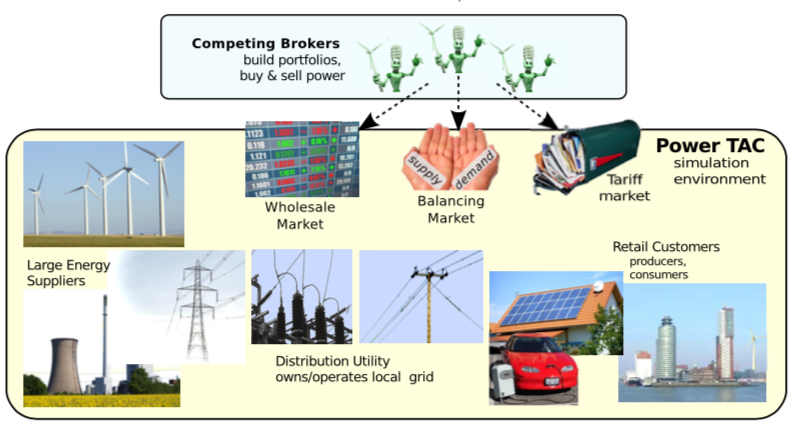
\includegraphics[width=1.0\textwidth]{powerTACScenarioOverview.png}
    \caption{An overview of the markets simulated in PowerTAC, from \citep{ketter2018powertac} }
    \label{fig:powertacoverview}
\end{figure}


%OVERVIEW,Economical
The broker to be developed has to contest in a number of markets and handle a variety of customer types. While
\ac{PowerTAC} generates a fairly complex landscape, it mostly aims at economic complexity rather than
modeling the technical underpinnings of the system. Therefore, it doesn't simulate any hardware but rather focuses on the
different agents involved in the market.

Its goal is to explore numerous market designs to correctly incentivize the market participants, allowing future
energy grids to be distributed, failure tolerant and adaptable to network dynamics \citep{ketter2015competitive}. Future
grids need to handle the changing landscape of energy production, delivery and consume patterns, triggered by the
increase of renewable energy sources and the planned reduction of fossil fuel dependency in many countries
\citep[p.13]{smartgrids2012smartgrids}.  

\subsection{Similar research}% \label{sub:similar_research}

\ac{PowerTAC} is part of a larger body of research focusing on agent-based simulations. The current landscape of generic
agent based simulation frameworks is summarized by \citet{abar2017agent}. \ac{PowerTAC} falls into a subcategory of
simulations concerning the energy markets. \citet{zhou2007agent} surveyed a number of tools in 2009, before the
inception of \ac{PowerTAC}. They define six categories to be used to compare a number of existing platforms and
frameworks for creating simulations. In this work, focus is placed on the components \ac{PowerTAC} does or does not
exhibit without describing the other platforms. \ac{PowerTAC} mostly focuses on the intermediaries between the end
consumers and the producers of energy, simulating both ends of the market through automated models and not by defining
them as agents with goals and intelligent behavior. It also does not simulate the transmission infrastructures and their
capacities, nor does it assume hierarchical structures of local and inter-regional grid interaction. \ac{PowerTAC} offers,
in the form of the central server instance, a strong "Independent System Operator", i.e.\ an instance that manages the
grid, the market and the communication between all agents in the simulation. The wholesale market deploys mostly
bidding approaches, in contrast to other simulations that also support bilateral mid- and long-term contracting options.
However, it emphasizes the concept of offering balancing capacity through energy storage devices and curtailment of
energy consumption which was not noted in the survey by \citet{zhou2007agent}.

\ac{PowerTAC} follows a distributed research approach. Teams can create their own agents and compete with each
other. This creates a rich landscape of solution approaches from researchers based in a number of countries and with
diverse backgrounds \citep{ketter2015competitive}. There is one drawback: few teams have opened their agents
implementations to others which increases the entry barrier and may lead to duplicate efforts that could have been
reused \citep{boettiger2015introduction}.

\subsection{Components}%
\label{sub:components}



\ac{PowerTAC} is both technically and logically separated into several components to aid both comprehensibility of the
system and yet allow complex simulations of more realistic scenarios. In the following pages, those logical components
will be explained. Most of these components are easily mappable onto the technical implementation. The technical
structure will not be explained in detail but can be found under the GitHub \ac{PowerTAC}
organization\footnote{\url{https://github.com/powertac/}}.


\subsubsection{Distribution Utility} The \ac{DU} represents an entity that regulates the real-time electric usage and
corrects any imbalances in its brokers portfolios. Any broker who did not balance its electric supply and demand incurs
costs and this works as an incentivize to always balance its portfolios as good as possible. The \ac{DU} also owns the
distribution grid and every broker must pay fees for the use of the grid in proportion to the volume of its customers
energy \citep[p.10]{ketter2018powertac}. Fees for the grid are constructed in a way to incentivize
brokers to not only balance their portfolio but also to avoid high peak demand. It further offers tariffs and it is
thus the equivalent of a \emph{baseline broker} whose tariffs define an upper bound on broker profitability.

\subsubsection{Accounting} All accounting is managed by the central simulation server to avoid adversarial brokers
from tampering with the games rules. Negative balances are usually punished with a 10\% p.a.\ interest rate while
positive balances receive a 5\% p.a.\ interest rate. This component tracks every broker's financial balance as well as
all brokers' customer subscriptions and wholesale market positions \citep[p.11]{ketter2018powertac}.

\subsubsection{Wholesale Market}
%TODO energy or electricity? What's the "right" word? --> ENERGY
Every broker needs to purchase energy before it can sell it to the customers unless such customers themselves
generate sufficient energy to balance the broker's own portfolio. For this, \ac{PowerTAC} offers a wholesale market that operates
a \emph{periodic double auction} which represents traditional energy exchanges like those existing in the United States
and European markets. Participants in this wholesale market are brokers as well as a large general entity
representing a number of generating facilities, a grid buyer who simulates large-scale demands based on real-world data
adjusted based on weather-forecasts and a wholesale buyer who regularly places high-volume, low-price bids. During each
time slot, 24 future slots are open for placing bids by the brokers. After the bids have been collected, a clearing
price is calculated which is the intersection between supply and demand curves. Orders without limit prices are
always served first. After the clearing, all uncleared bids and asks are disclosed and distributed to the brokers to indicate the
direction of the markets' demand and supply curves \citep[p.21f.]{ketter2018powertac}.

\subsubsection{Balancing Market}
The Balancing market is the last and final trading opportunity for agents and in the
sense of the game it occurs right after the last opportunity to trade for a target time slot meaning that it occurs
virtually in parallel to the consumption of electricity. Any imbalance during this phase is corrected by the \ac{DU} who
imposes forced balancing of brokers with an imbalanced portfolio. As a
result, brokers with too much supply in their portfolio receive very little reimbursement for it and those whose customers' usage is higher than the estimated amount pay
high prices for the additionally supplied energy. The \ac{DU} also distributes the cost for the grid infrastructure
according to the peak demand distribution among all brokers. This is based on the assumption that the grid
infrastructure has a static capacity equivalent to the maximum
transmission demands. Brokers are incentivized to create portfolios that don't exhibit large deltas between
different hours of the day or days of the week.

Moreover, those who have tariffs with economic control abilities can pass this capacity along to the \ac{DU} which uses
them to correct the markets imbalances, charging customers' storage devices if an oversupply is present or
depleting their devices in case of an undersupply. It is hence economically beneficial for brokers to attract
customers with such balancing capabilities since it offers a buffer capacity against the balancing costs otherwise
incurred through the actions of the \ac{DU} \citep[p.5]{ketter2018powertac}.

\subsubsection{Customer Market}

The foundation for any brokers' ability to generate profit is a sufficient amount of customers being subscribed to its tariffs. For
this to occur, the broker must publish tariffs that are competitive to attract customers. Nonetheless, if the
broker offers tariffs that lead to net losses, long term profit will not be possible\footnote{While the 2017
    competition technically allowed for brokers to remain in the game despite offering highly under-priced tariffs that
    corrupted the simulation results, a proper broker must not pursue such strategies due to economic
reasoning.}.

The broker has a wide variety of actions at its disposal to create a rich portfolio. The simulation offers the
creation of a variety of tariff types that have variables which are adaptable by the broker. The types include:

\begin{description}
    \item[Flat rate] Customers pay a flat rate per kWh and they always receive their demanded
        amount.
    \item[Tariff with fixed fee] Customers pay a definable fixed fee every day to receive the service.
    \item [Tiered rates] Customers pay a certain price per kWh until a limit is reached after which the kWh price
        changes.  Arbitrarily many such tiers can be added.  
    \item[Time-of-use] Customers pay different prices depending
        on the time of the day or the day of the week.  
    \item[Dynamic Pricing] Allows the broker to dynamically adapt the price per kWh in real-time to incentive customers
        to reduce their usage during high demand times. A minimum, maximum and mean price per kWh as well as a
        notification interval needs to be specified.
    \item[Curtailable] Customers can opt in to a tariff that allows the broker to reduce the delivered amount of
        electricity per time slot up to a certain percentage. This means the customer is exposed to a risk of not
        receiving the entire electrical supply demanded, usually for a discounted unit cost per kWh.  \item[Storage]
        Customers can offer their storage capacity to brokers to allow them to balance their portfolio. Customers
        receive payment from the brokers if their storage devices are being depleted and pay a (reduced) fee for charging
        events.
    \item[Signup fees and withdrawl fees] Customers can receive bonuses or pay fees
        for signing up or canceling a subscription.
\end{description}

\noindent Some of the above types can also be combined to create complex tariff landscapes for customers to choose from \citep[p.9]{ketter2018powertac}.

\subsubsection{Customer models}% \label{sub:customer_models}

The final part of the simulation environment is made up by the customer models which simulate real-world customers.
Each customer can both produce and consume electricity. Consumers are modeled both by factored and elemental models
\citep[p.14]{ketter2018powertac}, allowing for small numbers but detailed patterns and large number averaged
patterns respectively. The customers evaluate the offered tariffs based on a number of deterministic functions
including the various costs and variants of the offered tariffs multiplied by an \emph{irrationality factor} that
allows for a more realistic limited rationality of the actors. Additional assessments such as broker reputation
evaluation and energy source preferences are also included in the utility function.

Customers evaluate new tariffs irregularly based on an \emph{inertia factor} that limits
their attention to such tariffs. Customers are not inherently loyal to their brokers but the inertia factor
indirectly causes them to not immediately switch if there is a more rational tariff available.

As previously noted, customers can both consume and produce electricity. While most production is non deterministic
and non controllable (i.e.\ in the case of solar and wind electricity), some are controllable such as \ac{CHP} or
bio-gas units \citep[p.16]{ketter2018powertac}. Devices such as electric vehicles or water heaters can also offer
regulation actions allowing brokers to balance their portfolios. A \emph{smart} water heater could refill only minimally
after heavy use if usage patterns show that the owners will most likely not use it again for several hours. This
way, an additional, possibly profitable capacity for energy consumption is created for the consumer, as the broker
usually charges less for electricity delivered under capacity regulation terms \citep[p.14ff.]{ketter2018powertac}.

\subsection{Existing broker implementations}%
\label{sub:existing_broker_concepts}
Before designing an agent, it is helpful to investigate previously developed agents and their design to understand
the current state of research. For this, the papers of the brokers AgentUDE, TacTex and COLDPower were analyzed, because they
performed well in previous tournaments and because their creators have published their concepts. The
paper by \citet{peters2013reinforcement} was also analyzed as it was the first paper to describe a \ac{RL} agent acting in a predecessor
of the \ac{PowerTAC} environment. This broker, while technically not competing in the \ac{PowerTAC} competition, is
referred to as \ac{SELF}. Their architectures,
models and performances are summarized in the following pages. The analysis is based on publications that describe the
TacTex, COLDPower and AgentUDE agents of 2015, as they are the last publications of these brokers that are available on
the \ac{PowerTAC} website. Unfortunately, the source code of the agents has not been made available, which does not
allow inspection of the exact inner mechanics.

From what is visible by their shared binaries, all agents are based on java and do not employ any other technologies to
perform their actions during competitions.

\subsubsection{Tariff market strategies}%
\label{ssub:tariff_market_strategies}

AgentUDE deploys an aggressive but rigid tariff market strategy, offering cheap tariffs at the beginning of the game to
trigger competing agents to react. It also places high transaction costs on the tariffs by making use of early
withdrawal penalties and bonus payments \citep{ozdemir2017strategy}. While this may be beneficial for the success in the
competition, it doesn't translate into real-world scenarios as energy markets are not a round based, finite game.

TacTex does not target tariff fees such as early withdrawal fees to make a profit. It also doesn't publish tariffs for
production of energy \citep{tactexurieli2016mdp}. TacTex has modeled the entire competition as a \ac{MDP} and included the
tariff market actions in this model. It selects a tariff from a set of predefined fixed-rate consumption tariffs to
reduce the action space complexity of the agent. Ultimately, it uses \ac{RL} to decide on its tariff market
actions, reducing the possible actions based on domain knowledge.

COLDPower also deploys \ac{RL} approaches with a Q-Learning based agent choosing from a range of predefined changes to
its existing tariff portfolio. It can perform the following actions: \emph{maintain, lower, raise, inline, minmax, wide,
bottom}. These describe fixed action strategies that have been constructed based on domain knowledge \citep{cuevas2015distributed}. The agent
is not \emph{learning} how to behave in the market on a low level but rather on a more abstract level. It can be
compared to an \ac{RL} agent that doesn't learn how to perform locomotion to move a controllable body through space but
rather one that may choose the direction of the walk, without needing to understand \emph{how} to do it. While this
leads to quick results, it may significantly reduce the possible performance as the solution space is greatly reduced.

\ac{SELF} also defines the tariff market as a \ac{MDP} and uses feature selection and regularization to reduce the state
space of their learning \ac{SARSA} agent. The action space has been defined with discrete pre-defined actions that are
similar to the ones of the COLDPower agent \citep{peters2013reinforcement}. As COLDPower, the discrete action space by itself introduces assumptions about
the problem domain that the agent cannot overcome. As an example, the two actions \emph{LowMargin} (10\% margin) and
\emph{HighMargin} (20\% margin) restrict the profitablity of the agent to two points in the overall action space. Maybe
the optimum is at 14.25\% or maybe it is even higher than 20\%. A discrete action agent cannot discover nor act upon
these possible improvements. Neural networks may help overcome this limitation because they can both handle large state spaces
and act successfully in continuous state spaces.



\subsubsection{Wholesale market strategies}%
\label{ssub:wholesale_market_strategies}


AgentUDE's strategy for the wholesale market includes both demand and price prediction. For the demand prediction, AgentUDE
uses a simple weighted estimation based on the previous time-step and the demand of 24 hours before the target time-step
\citep{ozdemir2015winner}. Their price prediction is more complex and involves a dynamic programming model based on
\citep{tesauro2002strategic} to find \emph{similar hours} in recent history and determine current prices using
Q-Learning \citep{ozdemir2017strategy}. Their \ac{MDP} is constructed in a way that the agent needs to determine the
limit price that minimizes costs. It only has one action dimension which describes the limit price and its environment
observation is represented by a belief function $f(s,a)$ which makes it a \ac{POMDP}. The agent uses value iteration to
solve the Bellman equations, determining the expected price. The ultimate limit prices are then determined based on a
heuristic that works by offering higher prices for "short-term" purchases and adjusting this to also offer higher prices
in the case of an expected higher overall trading volume \citep{ozdemir2017strategy}.

TacTex considers the wholesale market actions to be part of the overall complexity reduced \ac{MDP}. It uses a demand
predictor to determine the \ac{MWh} amount to order and sets this amount to be placed in the order. The
predictor is based on the actual customer models of the simulation server itself. While this surely leads to good
performance, it can be argued whether it is something that actually benefits the research goal. The price predictor is
a linear regression model based on the bootstrap period, corrected by a bias correction based on the prediction error of
the last 24 hours \citep{tactexurieli2016mdp}.

COLDPower deploys a linear regression model to predict prices and determines the demand by "using the energy demand
historical information" \citep{cuevas2015distributed}. The order is placed accordingly.

The authors of \ac{SELF} don't describe its actions in the wholesale market. Probably, the early variant of the
simulation did not contain this component yet and simply calculated the market price for the
electricity to then submit it to the agent.


\subsubsection{Past performances}%
\label{ssub:past_performances}

To analyze the performance, all cash statistics of the final rounds of the year 2017 were analyzed. TacTex did not
participate in the 2017 competition, therefore it is excluded in this analysis. Their last participation was in 2015
where they ended up in second place. The improvements made to the previously mentioned agents between their latest
publications and their current performances are unfortunately not determinable.
\begin{figure}[]
    \centering
    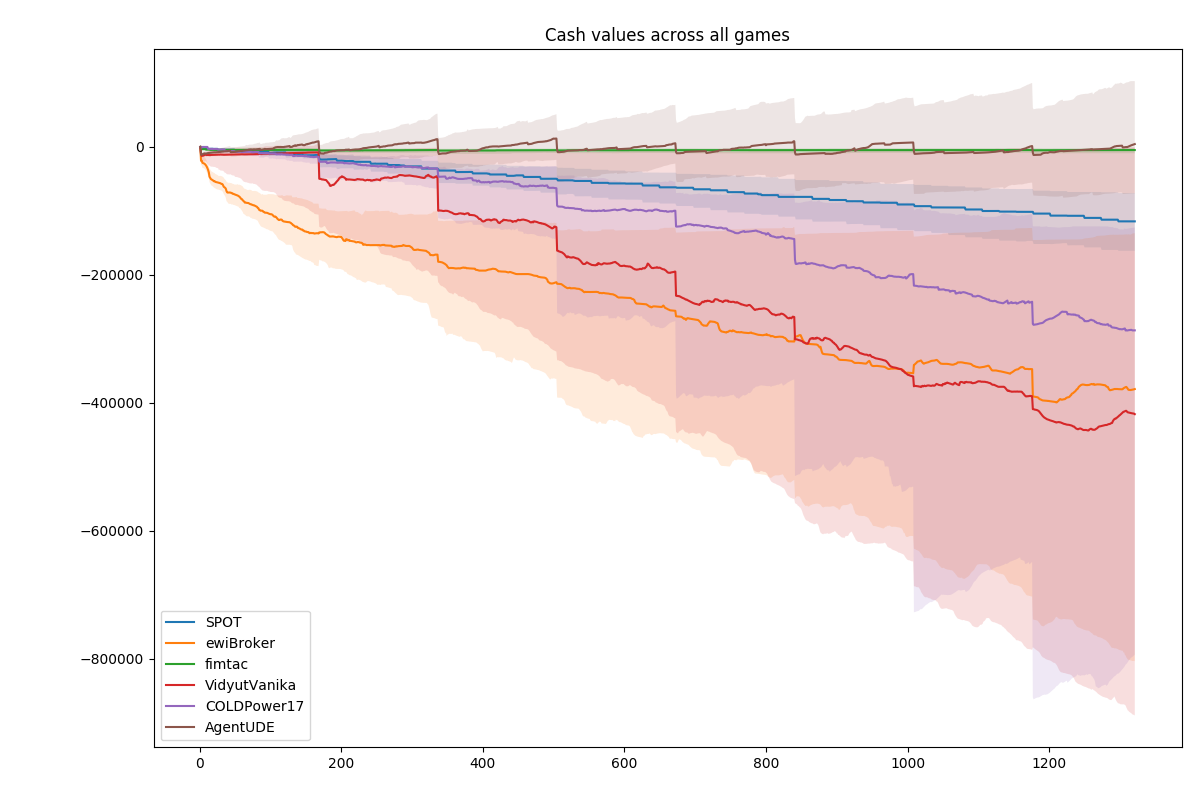
\includegraphics[width=1.0\linewidth]{img/cash_vals_across_games.png}
    \caption{Cash values across all games in the 2017 finals (median, 0.25 percentile, 0.75 percentile)}
    \label{fig:cash_vals_across_games}
\end{figure}

When looking at the overall performance profiles (see Figure~\ref{fig:cash_vals_across_games}) of the top 6 brokers of
the 2017 finals, it becomes obvious that most brokers are performing rather bad most of the time. Only SPOT, fimtac and
AgentUDE managed to consistently stay close to zero or in the case of AgentUDE even above a 0 cash balance. When
inspecting the tariff transactions closer (see Figure~\ref{fig:allttxucline}), it becomes clear that only AgentUDE
achieves this through actually being successful in the market. SPOT only acts in the market initially and then quickly
looses many of its customers. Fimtac keeps a small continuous customer base throughout most games. AgentUDE on the other
hand trades actively in the market, having a solid number of customers subscribed to it.  COLDPower also trades actively
but its financial results are not as satisfying, loosing significant amounts of money each week and also not being able
to sustain its continuous income towards the end of the games.
\begin{figure}[]
    \centering
    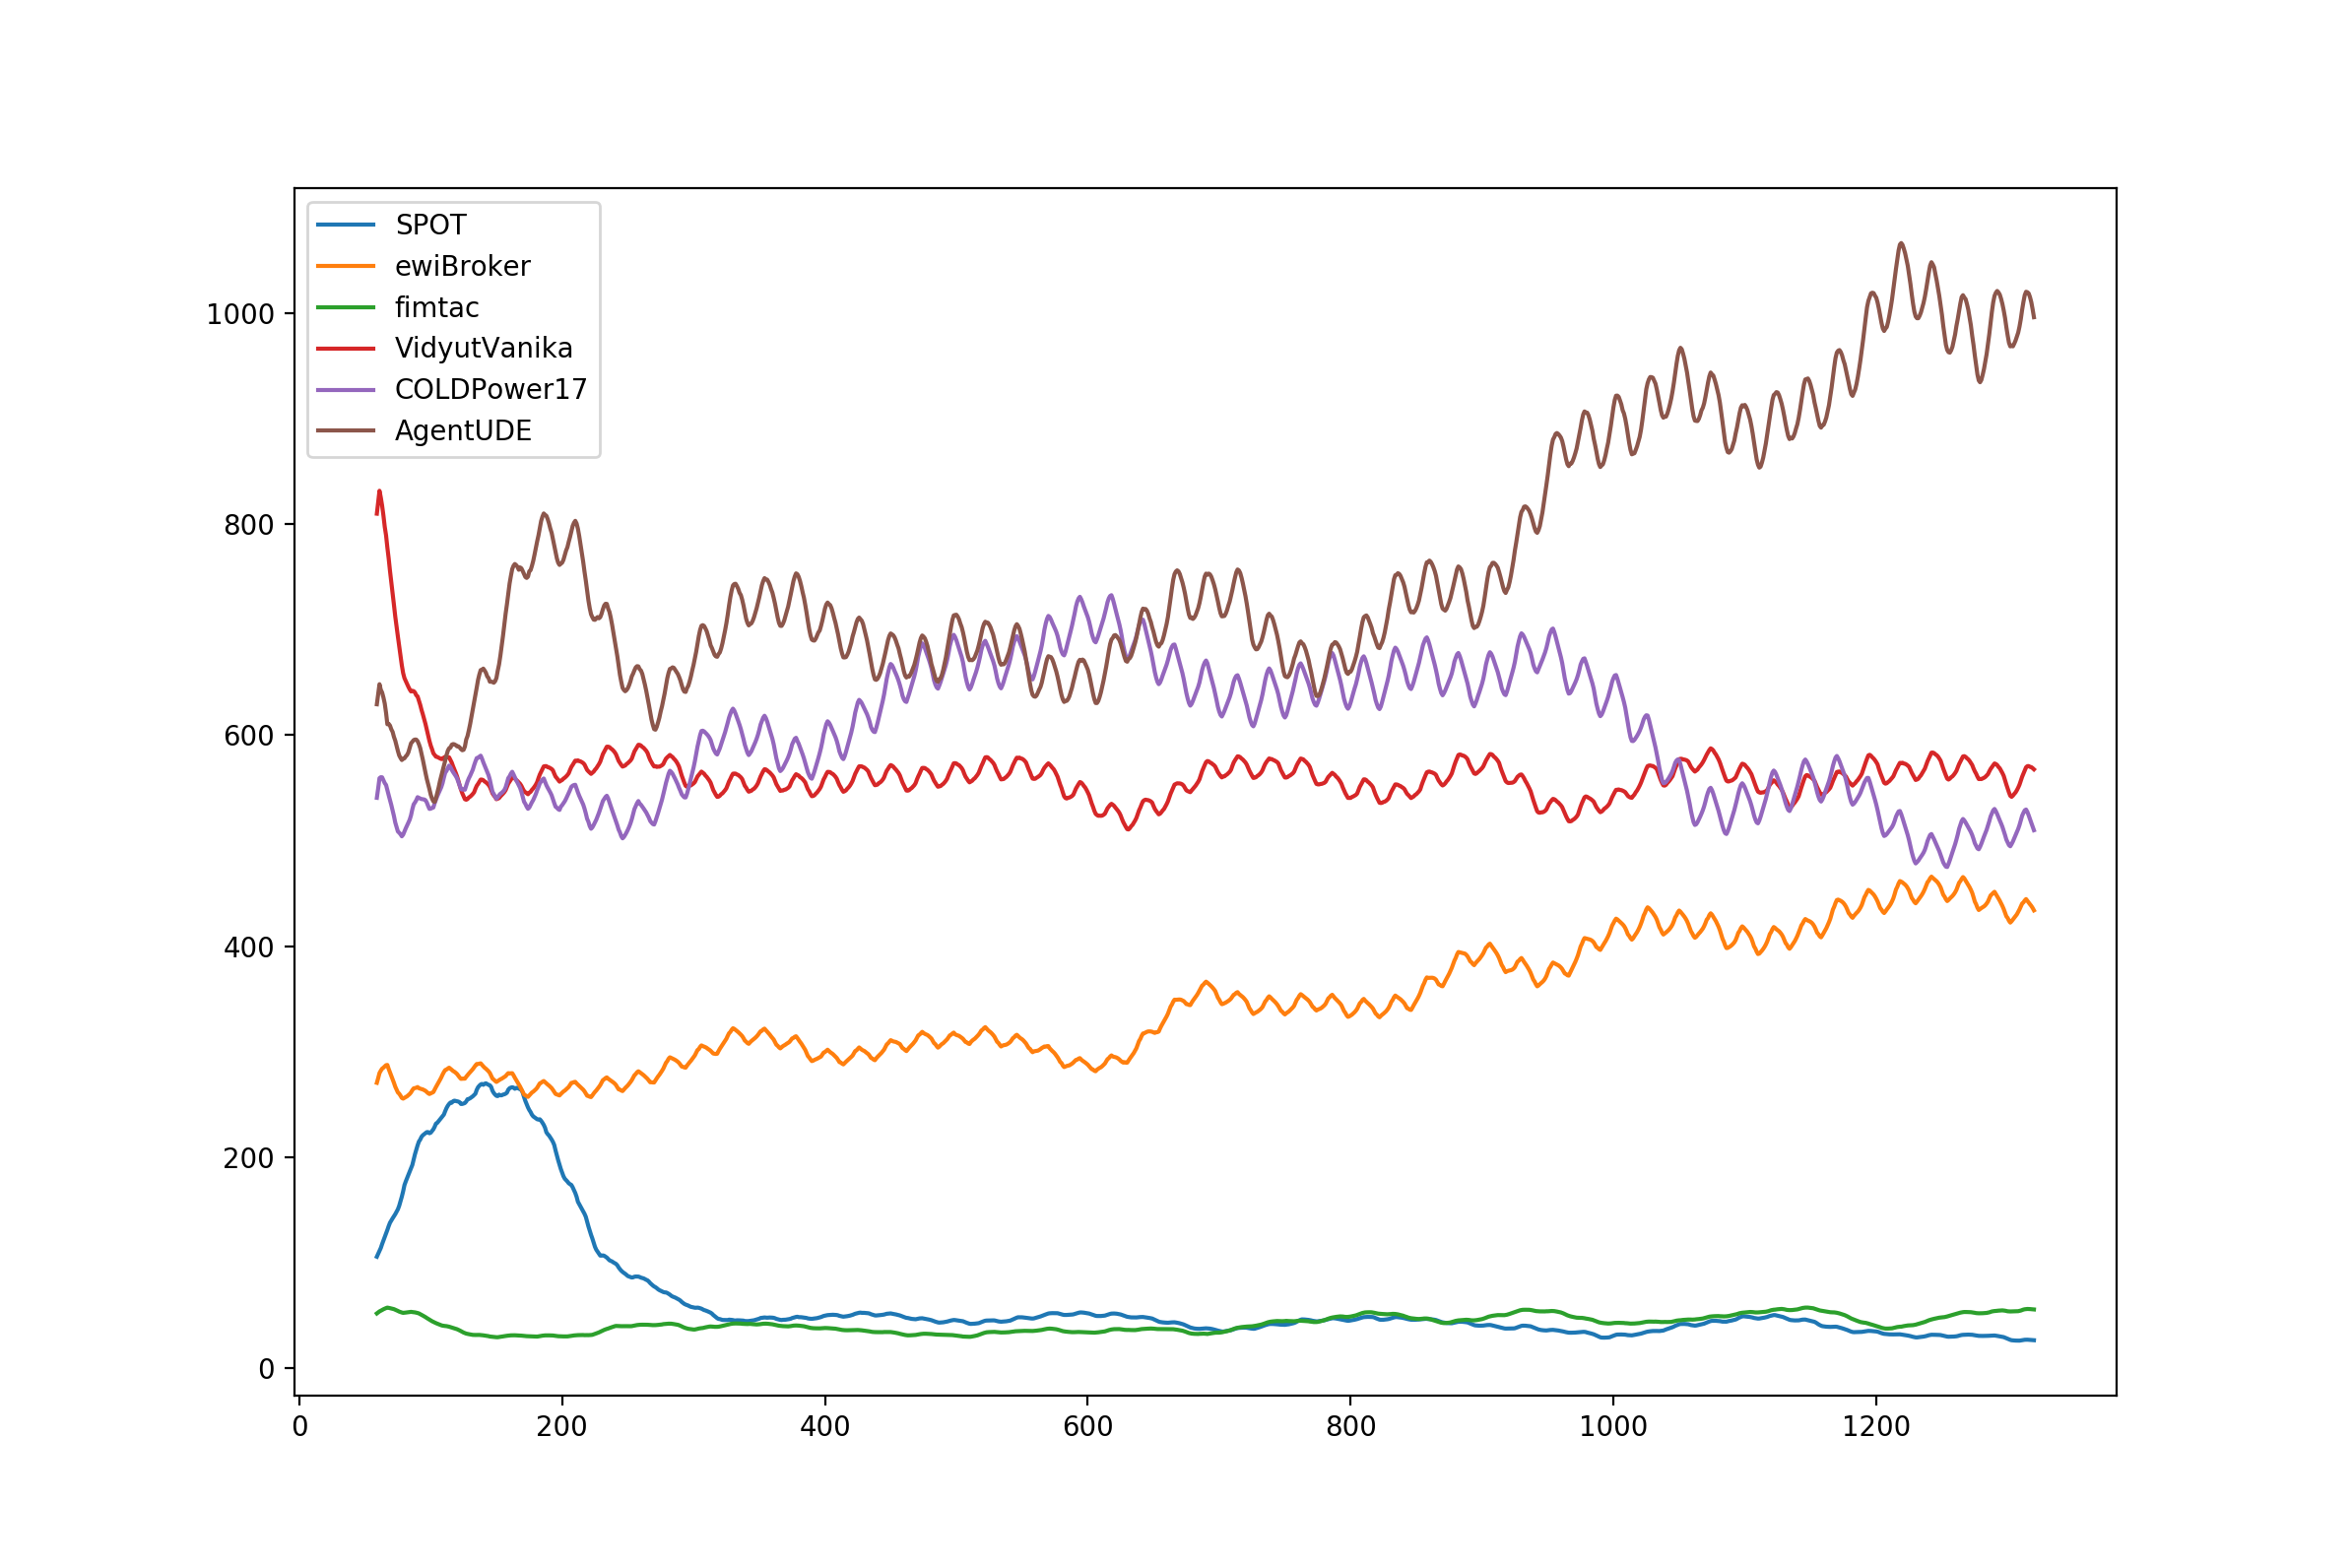
\includegraphics[width=1.0\linewidth]{img/all-ttx-uc-line.png}
    \caption{Tariff TX credit values across all games in the 2017 finals (rolling average)}
    \label{fig:allttxucline}
\end{figure}

Generally, AgentUDE can be seen as the peer with the best and most stable performance. Their broker acts in all
parts of the simulation and makes use of various strategies, including tariff optimization and balancing capacity.
Importantly, it is still taking part in the competition as of 2018.

\section{Applying observation learning to PowerTAC}%
\label{sub:applying_observation_learning_to_powertac}

This section describes concepts that may be pursued in the development of more performant brokers for
\ac{PowerTAC}. They all adhere to the idea of learning from either previously recorded actions of other brokers or by
observing other brokers in the environment.

Generally, a neural network based policy function or value function requires a significant amount of training.
Similarly, supervised learning problems require a large training dataset to converge onto their potential performance.
Running a simulation takes about 3 hours (due to its fixed time slot length of 5 seconds) and delivers some 1600
training steps. This is far below what supervised learning algorithms can train on in a given time span and also \ac{RL}
agent algorithms can perform several hundred steps a second on contemporary hardware. When accelerating the training of
the network using modern \ac{GPU}, this discrepancy becomes even more significant. For the \ac{RL} based wholesale
trading component, some techniques can be applied to boost its learning performance either through offline learning
prior to have it interact with a live environment or by increasing the sample efficiency through transfer learning
methods. These techniques are described below.

\subsection{Offline wholesale environment approximation}%
\label{ssub:offline_record_based_wholesale_environment_approximation}

\ac{PowerTAC} allows developers to download large amounts of historical game records. Several hundred games are
available for 2017 alone, all with different broker participants and broker counts. The \texttt{powertac-tools}
repository makes it convenient to download all  of them and analyze them for specific data, providing csv files for
further analysis. Using the \texttt{powertac-tools} project for all games downloadable for 2017, records were created to
let the broker train on the datasets. The \texttt{CustomerProductionConsumption.java} file
provides a historical dataset that can be used to create a hypothetical portfolio for the learning \ac{RL} agent. To design a \ac{RL}
environment, the broker needs a realistic portfolio of required energy. Therefore, a subset of the customers may be
chosen to pose as the brokers portfolio. While in a real simulation setting, the customers constantly join and leave
brokers tariffs, this offline environment approximation would assume a static portfolio. Furthermore, the market prices
analysis\footnote{\texttt{MktPriceStats.java}} gives a historical record of all market closings for each game. In a
historical data based environment approximation, the market prices are not influenced by the brokers placement of ask
or bid orders. This is unrealistic if the broker represents any significant percentage of the overall market but may be
a good approximation if the portfolio of the broker is only covering a small percentage of the market. Ultimately, this
environment allows for rapid training of a \ac{RL} agent in the \ac{PowerTAC} environment by approximating its wholesale
market. The disadvantage is the fact that it's an approximation of the later simulation environment. The improved learning speed
is caused by the agent not having to wait for the server to inform it about a new open time slot. Instead, the
time slot is artificially stepped whenever the wholesale trader has completed its trades. This approach is the one
chosen for the later implementation of the wholesale trading agent.

\subsection{Learning from recorded teacher agent actions}%
\label{ssub:learning_from_historical_actions_of_teacher_agents}

The \ac{RL} agent may in addition to a fixed portfolio be taught to imitate the recorded behavior of a teacher broker
such as a former winner of the competition. It may be given the recorded demand data of a competing broker and the
reward function would be modeled in a way that incentivizes the agent to behave similar to its teacher broker. This is
in accordance to the concepts of inverse reinforcement learning. If the broker may also act in a live competition, it
could implement the kickstarting concept of \citet{schmitt2018kickstarting}, feeding its observations to a competitor
teacher broker and initially attempt to align its actions to those of the teaching broker. Unfortunately, the latter concept
is difficult to implement in the \ac{PowerTAC} environment. Brokers are black boxes and it is not possible to assume
that they will behave correctly if their submitted actions are not the ones actually submitted to the server (due to
replacing them with those of the learning agent). This would be required, since the learning agent is the one that
actually determines the policy by giving its observations to the teacher agent asking for its \emph{opinion}.
\citet{schmitt2018kickstarting} model lets the agent consider the question of what its teacher would do if it were in
its situation. Due to the inaccessibility of the teaching brokers inner workings, an alternative model could only ask
\emph{what would I do if I were in my teachers situation}. To allow for such analysis, the next technique is required.

\subsection{Counterfactual analysis}%
\label{ssub:counterfactual_analysis}

Many real-world problems are approachable with \ac{RL} agent research. What makes \ac{PowerTAC} and other simulations
interesting is the ability to perform counterfactual steps. A counterfactual event is one that is not aligned with what
is actually true. In a real scenario, the statement \emph{"Alan Turing would have not cracked the Enigma encryption if he
had been fed one apple a day by his mother every morning"} is (probably) against what is actually true and consequently cannot
possibly be verified. In the \ac{PowerTAC} simulation, this is different. Because the entire state of the server is
recorded in its state files, it can be reproduced exactly. Unfortunately, the brokers do not offer such ability to
reproduce their state. A level of randomness is inherent in their decision making. If a statement were to be: \emph{"If
the broker had offered tariff X in time slot 1200, it would have won the competition"}, it is not sufficient to reproduce the
state of the server from the state files alone to verify this hypothesis, because of the randomness of the brokers.

With a technology that allows for \emph{snapshotting} of memory space in Linux, it is possible to create a snapshot of
the server state and all its participants running on the same machine \citep{criu}. A broker developer may thus leverage the
ability to create a snapshot of the entire environment state to evaluate a number of alternative actions at any point
within the game instead of having to rerun an entire simulation. This approach does not require all broker developers to
support this feature. Instead, the mentioned technology allows \emph{any} process in the operating
system to be stored and recreated being in the exact same state as before. This means, a \ac{RL} agent cannot learn simply
through performing full episodes within a learning session, slightly altering its behavior randomly within each episode.
Instead, the agent may decide to try all or a subset of the possible actions at any given moment to determine which of
the alternative actions leads to the highest rewards within a given time frame. The model would therefore be a bit
different from usual \ac{MDP} models which follow a iterative, non-branching concept. It would allow the agent to submit
a number of actions and ask the environment to give back a set of depending rewards. Conceptually, it is the equivalent
of the agent asking \emph{"which of these actions gives me the best reward?"} Applied to the \ac{PowerTAC} environment
it is still susceptible to random behavior \emph{after} the snapshot occurred (due to random number generators used or
other sources of entropy), but it is guaranteed to be the exact same state at the point where multiple actions are
considered. Remaining uncertainty may now be compensated by running a significant amount of trials ceteris paribus.

An experiment performed during the creation of this work has shown that such an analysis is
possible\footnote{\url{https://www.youtube.com/watch?v=10iqP9Zdi4U}} with \ac{PowerTAC}. Additionally, to allow a
researcher to control the flow of messages between the server and other agents (permitting the change of other agents
behavior), a modification of the powertac server which opens up all communications to a definable \emph{spy broker} has
also proved to work
\footnote{\url{https://github.com/pascalwhoop/powertac-server/commit/1f0455929e7062faf8617cd5ca6e6a138f250382}}. Yet,
the concept was not pursued further, as the creation of a broker framework and the enabling of current tools was
prioritized.

\section{Implementation }
\label{sec:implementation}

The following sections will describe concepts and reasons behind the various components needed to allow a broker to
leverage modern reinforcement learning tools and algorithm libraries in the \ac{PowerTAC} environment. Current
state-of-the-art algorithms for \ac{RL}, available mostly in Python \citep{baselines}, are used. These leverage the
TensorFlow and the Keras high-level abstraction libraries \citep{plappert2016kerasrl}.

%In general, a considerable amount of work was invested enabling communication between an agent
%written in Python and the \ac{PowerTAC} systems which are Java based. The preliminary research and its results are summarized in
%Section~\ref{sec:connecting_python_agents_to_powertac}. Because of this additional complexity, the practical part of the thesis was
%restructured to allow for successful contribution to the \ac{RL} field by performing a form of \emph{what-if}
%analysis in the wholesale market which is described in Section~\ref{sub:wholesale_market}. The Python environment has
%been constructed in a way to allow for future developers to leverage it as a framework for developing a fully capable
%agent that acts in all markets.

The overall architecture of the broker is composed of five main components: the communication abstraction, wholesale market
agent, balancing market agent, tariff market agent and demand predictor. In this implementation, only the wholesale
market and demand predictor are actively making decisions. Future researchers can make use of the component structure.
The architecture is visualized in Figure~\ref{fig:agentframework}.

While \citep{tactexurieli2016mdp} have defined the entire simulation as a \ac{POMDP} (interpreting it as a
\ac{MDP} for ease of implementation) with all three markets integrated into one problem, this work breaks the problem
into distinct sub-problems as each of them can be looked at in separation and a learning algorithm
can be applied to improve performance without needing to consider potential other areas of decision making. A
subsequent algorithm could then be trained to perform the same actions as one unified decision making system according
to the concepts of \emph{Curriculum Learning}\citep{matiisen2017teacher} and \emph{Transfer Learning}
\citep{parisotto2015actor}. Such steps require more advanced forms of machine learning architectures and should
therefore be approached in future work.
To justify this separation of concerns, one may refer to the estimation of fitness for a given tariff in a given environment.
A tariffs' competitiveness in a given environment is independent of the wholesale or balancing trading strategy of the
agent since the customers do not care about the profitability of the agent or how often it receives balancing penalties.
While the broker might incur large losses if a tariff is too competitive by offering prices that are below its
profitability line, this tariff would be quiet competitive in theory and should hence be rated
as such. The question concerning which of the tariffs is best to offer on the market is a separate problem that balances
competitiveness against profitability. Similar arguments can be made for the other components.

First, a number of tools used in the implementation are described as well as the preprocessing of the existing data
using both new and existing code. This is followed by a description of the new communication architecture for non-java clients.
Finally, the code behind the two implemented learning components, the demand prediction and the wholesale
trading agent will be described.

%The overall architecture for the agent is composed of three key modules.First, the environment module, which hosts all known
%information about the environment of the broker. This is used by all learning components. Second, A communication module
%bridges the environment module and the \ac{PowerTAC} environment to hide communication overhead from the agent code,
%letting the learning components access the environment as if it was not remotely defined.
%Third, the agent components module holds all learning components such as the wholesale trader, the demand estimator
%and the tariff manager. In the scope of this thesis, only the demand estimator and the wholesale trader were implemented
%but the framework allows for the additional components to be easily implemented. The architecture is visualized in
%Figure~\ref{fig:agentframework}.

\begin{figure}[t]
    \centering
    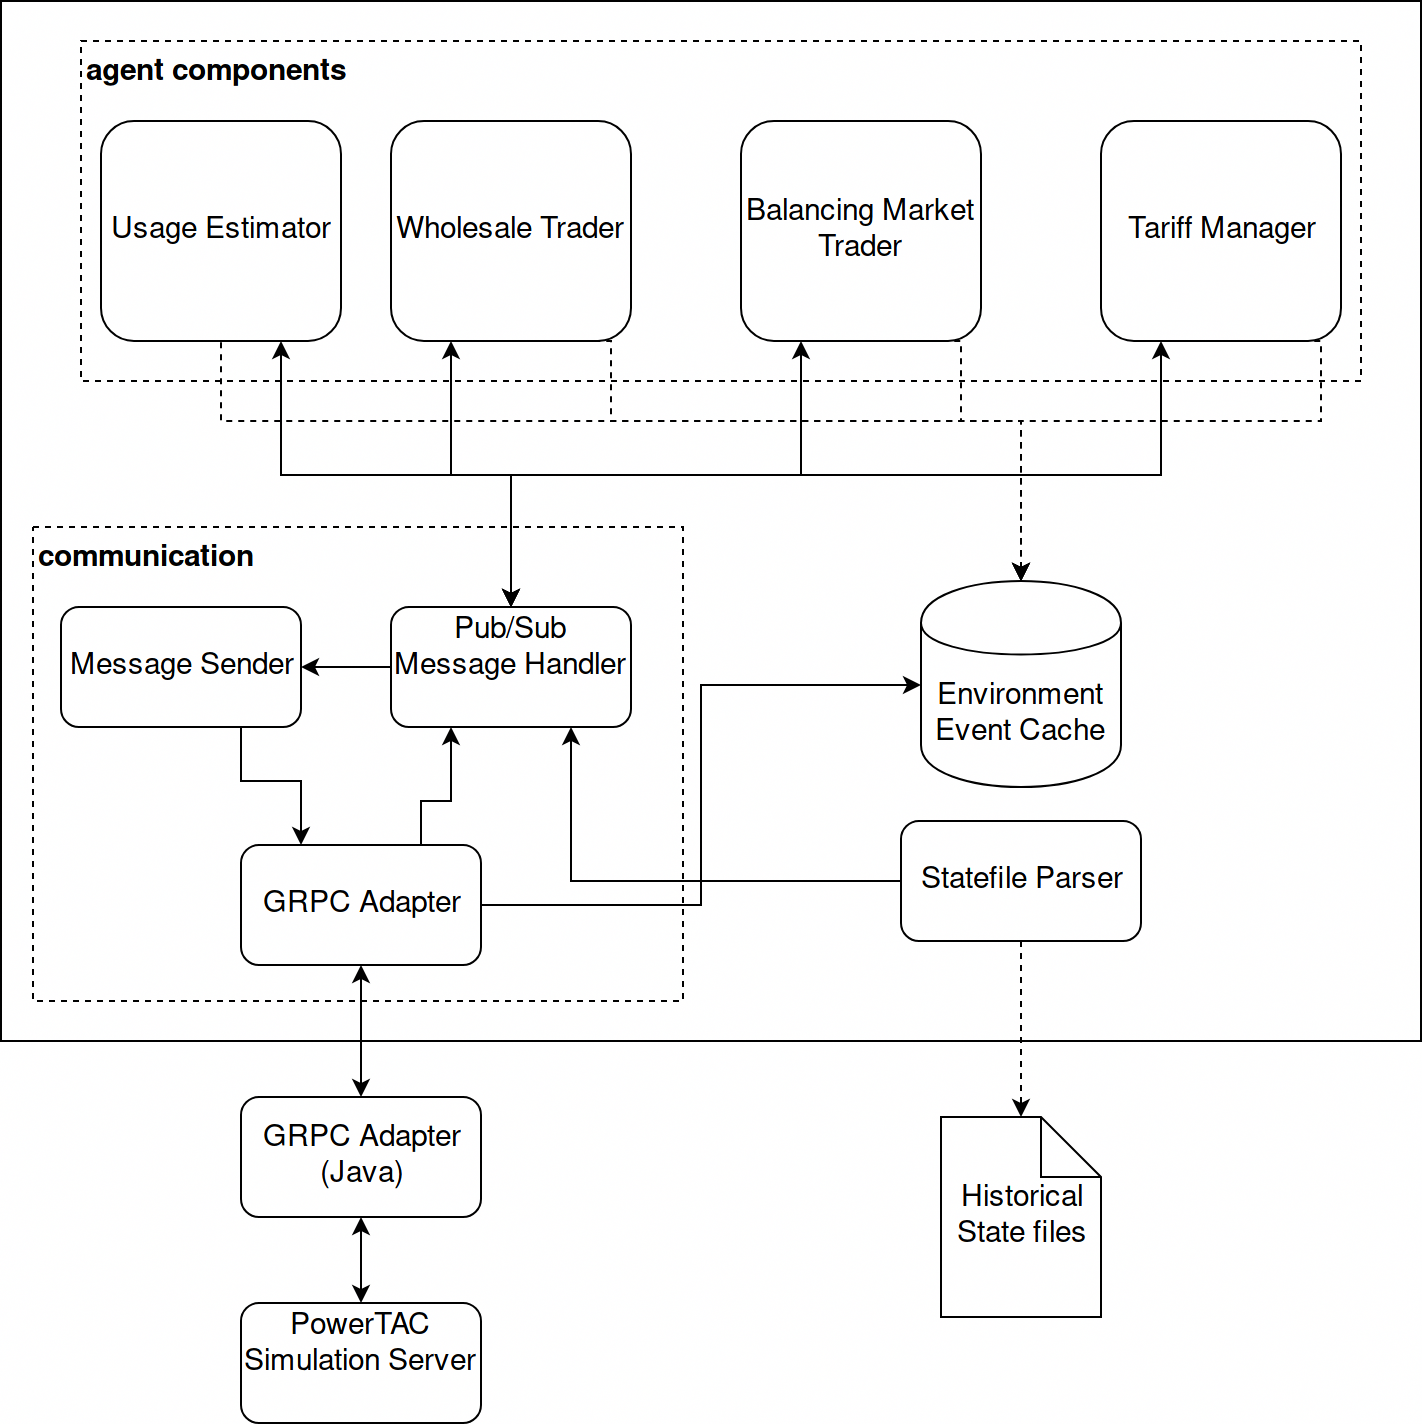
\includegraphics[width=1.0\linewidth]{img/Agent.png}
    \caption{Architecture of the python broker framework}
    \label{fig:agentframework}
\end{figure}


\subsection{Tools}

To develop the functionality of the agent, which is supposed to be mainly driven by deep learning technologies, a number
of state-of-the-art tools and frameworks were  used. These include
Keras and TensorFlow to allow for easy creation and adaption of the learning models,
\ac{gRPC} to communicate with the Java components of the competition and
\emph{Click} to create a \ac{CLI} that allows the triggering of various components of the broker.

%Kubernetes to easily scale several instances across the cloud.
%By transferring the components into the cloud, it is also
%possible to use tools such as Google Colab which allows access to a powerful cloud \ac{GPU} without costs


\subsubsection{TensorFlow and Keras}%
\label{sub:tensorflow_and_keras}

TensorFlow is a library developed by Google to facilitate machine learning algorithms. It can leverage both \ac{CPU}
and \ac{GPU} computing power which can significantly increase performance. It is Open Source, used in various
technologies and serves as a base technology for many higher level frameworks \citep{tensorflow2015-whitepaper}.

Keras is one of these higher level frameworks that focuses on neural networks. It offers an intuitive \ac{API}, oriented towards
neural network terminology to quickly develop and iterate on various neural network architectures. It integrates TensorFlow and its
accompanying \ac{UI} Tensorboard, which visualizes training, network structure and activation patterns. It also supports
other base technologies beside TensorFlow, but these will not be discussed. A simple example for a 2 layer Dense neural network written in Keras is shown in Listing~\ref{lst:kerasbasic}.


\begin{listing}
    \begin{minted}[linenos,numbersep=5pt,frame=lines,framesep=2mm]{python}
from keras.layers import Dense

model.add(Dense(units=64, activation='relu', input_dim=100))
model.add(Dense(units=10, activation='softmax'))
model.compile(loss='categorical_crossentropy',
              optimizer='sgd',
              metrics=['accuracy'])
# x_train and y_train are Numpy arrays -- just like Scikit
model.fit(x_train, y_train, epochs=5, batch_size=32)
loss_and_metrics = model.evaluate(x_test, y_test, batch_size=128)
    \end{minted}
    \caption{Basic Keras 2 layer dense neural network example}
    \label{lst:kerasbasic}
\end{listing}

\subsubsection{Tensorforce and keras-rl}%
\label{sub:tensorforce_and_keras_rl}

Tensorforce and keras-rl are both relatively young libraries that intend to offer a high-level \ac{API} for building
\ac{RL} agents. Keras-rl, as the name suggests, is based on the Keras library and includes a number of \ac{RL} agent
implementations such as Deep Q-Learning (discrete and continuous) and \ac{SARSA} \citep{plappert2016kerasrl}. Over the
last few months, the progress of the project has been rather slow and Tensorforce offers a rich alternative.
Although not based on the high-level Keras library, it offers configuration of architectures and hyperparameters via
\ac{JSON} files. Due to large changes in the TensorFlow library between versions 1.6 and 1.8, it is scheduled to be
replaced by a new framework called "YARL", but the \ac{API} will be similar\footnote{Information received during private
    correspondence with the authors, see also
\url{https://github.com/pascalwhoop/broker-python/issues/5}}. Although the initial \ac{RL} trials were based on
keral-rl, it quickly became obvious that another library named Tensorforce was more appropriate due to its higher
flexibility, better documentation, stronger developer activity\footnote{based on the GitHub project metrics} and most
importantly, because it allows for a reversal of process flow control as is needed for the
\ac{PowerTAC} environment.

\subsubsection{Click}%
\label{sub:click}

%TODO cite only name, year missing, not correct?
Click allows the creation of CLI interfaces in Python. Programs can be customized with parameters and options as well
as structured into sub commands and groups \citep{clickcli}. This allows for patterns such as \texttt{agent compete
--continuous} or \texttt{agent learn demand --model dense --tag v2}. An annotated function is shown in
Listing~\ref{lst:click_sample}.

\begin{listing}[h]
    \begin{minted}[linenos,numbersep=5pt,frame=lines,framesep=2mm]{python}
@cli.command()
@click.argument('component', type=click.Choice(AGENT_COMPONENTS))
@click.option('--model', help="omitted in paper")
@click.option('--tag', help="omitted in paper")
def learn(component, model, tag):
    """Triggers the learning of various components
       off of state files"""
    if component in cfg.AGENT_COMPONENTS:
        component_configurator = get_learner_config(component)
        component_configurator.configure(model, tag, True)
        instance = component_configurator.get_instance()
        instance.learn()
    \end{minted}
    \caption{Click sample declaration}
    \label{lst:click_sample}
\end{listing}

%\subsection{CRIU}%
%\label{sub:criu}
%\ac{CRIU} allows the freezing and storage of an application during runtime. This permits what is an equivalent of a fork
%of the \ac{PowerTAC} simulation in a given point in time. Because \ac{CRIU} is also integrated into Docker, creating
%containers for various components of the competition (i.e.\ server and brokers) and freezing all of them in a coordinated
%manner is very helpful. This allows for two "what if" scenarios to play out at a given point in time where the results
%can be compared \citep{criu}. A typical scenario for the technology is the live migration of running applications across
%server infrastructures. In theory, a checkpoint of an application allows the perfect recreation of the application state
%even after a complete reboot of the machine or the moving of the application to a different host with identical
%environment settings.

\subsubsection{Docker}
\label{sub:docker}

Docker creates isolated, transferable images that include everything an application requires to run. A docker image, the
main artifact produced by the tool, contains a complete operating system environment as well as any dependencies and
executables. An
image can be based on various operating system distributions and many containers, an executed image instance, can run on a single server without much overhead.
\ac{VM} technologies are often compared to containers, but \ac{VM}s abstract on a different layer. A \ac{VM} simulates
an entire operating system on top of a layer called the hypervisor. Instead, Docker only abstracts the application
layer, letting all containers run in the same kernel, therefore it makes use of the existing resources in a more
efficient way. Nonetheless, it allows the creation of portable infrastructure components
\citep{boettiger2015introduction, docker}. This may be helpful if brokers become more complex, require more
technologies or simply to allow new developers to quickly get started with a competition environment. Docker has been
described as a means to improve portability and sharability of research artifacts and the tool has been widely adopted
in the software engineering industry to improve operations of continuously changing information systems
\citep{boettiger2015introduction}.
%Because \ac{CRIU} is integrated into Docker\footnote{at the time of writing, CRIU support is experimental in Docker},
%containers can be stored to disk using the \emph{checkpoint} feature.

\subsubsection{\acl{gRPC}}%
\label{sub:grpc}

\acf {gRPC} is a remote procedure call framework developed by Google Inc. It allows various languages and technologies to
communicate with each other through a common binary format called \emph{protocol buffers} or short \emph{protobuf}. All
communication can be encrypted via \ac{SSL}, offering
security and authentication. Over-the-wire data representation can either be binary or \ac{JSON}
\citep[]{grpc}. The benefits over the
current implementation are described in Section~\ref{sub:grpc_based_communication}. \ac{gRPC} is used by many machine learning
frameworks to allow distributed learning on many computing nodes \citep{tensorflow2015-whitepaper}.


\subsubsection{MapStruct}%
\label{sub:mapstruct}

MapStruct transfers data between Java objects of different classes. This problem is very common in large
software projects where domain objects may be outside the control of the developing team or based on external libraries.
If several components need to be integrated, translation is often necessary to adhere to the object structure required
by the library. MapStruct offers to generate otherwise manually created code based on best practices and naming
conventions. It is compile-time based, generating all code during compile time. This offers better error avoidance and
performance compared to alternatives that are reflection based
\citep[]{mapstruct}.
An example is given in Section~\ref{sub:implementing_the_communication_with_ac_grpc_and_mapstruct}.





\subsection{Connecting python agents to PowerTAC}%
\label{sec:connecting_python_agents_to_powertac}



To connect an agent based on Python to the \ac{PowerTAC} systems, a new adapter was developed. In early 2018, a simple bridge
was provided by John Collins, a member of the \ac{PowerTAC} team. It allowed external processes to communicate with the
system through a bridge via the provided sample-broker. All messages received by the broker were written to a First in
First Out pipe on the local file system and a second pipe was created to read messages from the external process. This
was the first approach towards opening up the simulation to other languages and development environments. Another
alternative approach would have been the creation of a function-specific adapter that only calls an external python
program to perform specific decisions\footnote{A comparing discussion can be found at
\url{https://github.com/powertac/powertac-server/issues/974}}.

Creating a complete communication adapter opens the doors for possible later migration of the technology to the server.
Using a highly performant technology instead of using \ac{XML} may also enable future competitions to scale to many more
competitors.Generally, the following problems needed to be solved:

\begin{itemize} \item Java model classes, or some language agnostic model description, should be reused if possible,
    automatically generating target language model definitions from the Java source code to avoid duplication of
    semantically identical information \item Permit future developers using even more languages (such as C, R or Go)
    with little effort \item Possibly lay the basis for a change of the communication technology of the entire
    simulation which is more language agnostic and performant
\end{itemize}

\subsubsection{Evaluating communication alternatives}%
\label{sub:evaluating_communication_alternatives}

After researching the current implementation and based on previous development experiences and current best practices,
the following three alternatives have been investigated in detail.


\paragraph{\acs {XML} via \acs {gRPC} }%
\label{sub:xml_via_ac_grpc}


The first approach is quiet similar to the original bridge but instead of writing the \ac{XML} strings to the local file
system, they are passed to the final environment via \ac{gRPC} by simple messages that serve as a wrapper for the
\ac{XML} string. While this is not elegant from a engineering perspective (\ac{gRPC} should be used on a method level
and messages should not contain other message formats as strings), it is simple and leads to quick results. A problem
is that the resulting \ac{XML} will then have to be parsed in the Python broker. Before the introduction of other
languages, the communication was implicitly an internal API and broker developers only needed to concern themselves with
the handling of the Java \texttt{handleMessage} methods. Therefore, no formal descriptions for the structure of the \ac
{XML} messages exist. All \ac{XML} parsing would thus be based on observable structures of the \ac{XML} which can
be extracted from the sample-broker logs and all model classes would need to be rewritten. Furthermore, agents wanting to use
other programming languages would have to reimplement all of this again, with little to no possible reuse.

\paragraph{True gRPC}%
\label{sub:grpc_based_communication}

A better but more complicated approach is based on \ac{gRPC} to transmit the messages between the Java sample-broker and
the final client, hooking into the \texttt{handleMessage} methods in the sample broker.
While previous developers have handled these messages in the Java environment, the adapter passes these messages to the ultimate
environment by converting them into protobuf messages which are then sent to a connected broker who implements
corresponding handler methods in the target language.

The advantage of this approach is that it allows the maintainers of the project to also adapt this approach for the
Java clients in general, massively reducing the communication overhead of \ac{XML} messages. The over-the-wire protocol
is much more
efficient (as the data is sent in a binary format) and the message structure is clearly documented in the
\texttt{grpc\_messages.proto} file. When serializing a \texttt{Competition} object, \ac{XML} requires 48 kByte while
the protobuf message is 14 kByte large, 70\%
smaller\footnote{\url{https://github.com/pascalwhoop/grpc-adapter/blob/master/adapter/src/test/java/org/powertac/grpc/mappers/CompetitionMapperTest.java\#L64}}.
When looking at the serialization and deserialization performance of \ac{XML} vs protobufs, a comparison of 1000
iterations of each operation for each variant also shows a significant improvement. While the deserialization of
protobuf messages performs about 5x less well (7444ms protobufs, 1366ms \ac{XML}), the serialization is 44x times
faster (1619ms \ac{XML}, 37ms
protobufs)\footnote{\url{https://github.com/pascalwhoop/grpc-adapter/blob/master/adapter/src/test/java/org/powertac/grpc/mappers/CompetitionMapperTest.java\#L90}}.
This can on the one hand be explained by the amount of string handling that \ac{XML} requires and on the other hand the fact that the
deserialization of protobuf messages includes a mapping of the binary format into the proper Java object via MapStruct instead
of using reflection. Generally, the server sends more messages than it receives, having to answer most messages and
redistribute information to all participants for any public information.


The disadvantage is the need to translate each \ac{POJO} into a protobuf message and
vice versa. This is, however, not different from the current XStream implementation which also requires the annotation of
class files in Java to declare which properties are serialized and included in the \ac{XML} strings. If the project
should adopt the \ac{gRPC} based communication, the \ac{gRPC} architecture will then allow the server to be addressed by any of the supported languages\footnote{Which as of today are: C++, Java, Python, Go, Ruby, C\#, Node.js, PHP and
Dart}. Using MapStruct as a mapping tool also makes the mapping structured. By performing round trip tests of the
transformed elements, it can be assured that the transformations between protobuf messages and \ac{POJO} perform as
expected\footnote{\url{https://github.com/pascalwhoop/grpc-adapter/blob/master/adapter/src/test/java/org/powertac/grpc/mappers/AbstractMapperTest.java\#L54}}.



\paragraph{JSON schema based communication}%
\label{sub:json_schema_based_communication}


A final approach is the generation of schema definitions from the Java model classes that are transmitted between the
brokers and the server. This formalizes the currently informal \ac{XML} \ac{API}. In general, two human readable
over-the-wire structures are reasonable: \ac{XML} and \ac{JSON}.  \ac{XML} messages can be formally defined using
\ac{XML} Schemas and the \ac{JAXB} project\footnote{\url{https://github.com/javaee/jaxb-v2}} offers to generate such
schemas from Java class definitions. This, however, did not succeed for the \ac{PowerTAC} model definitions which lead
to the creation of a question on StackOverflow, a discussion platform for programming questions. The resulting answer
inspired the ultimate alternative which is the generation of \ac{JSON} schemas that can then be converted into Python
class
files\footnote{\url{https://stackoverflow.com/questions/49630662/convert-java-class-structures-to-python-classes/49777613\#49777613}}.
The choice of \ac{JSON} as the base communication protocol might also be intelligent as a future choice two reasons:
firstly, it seems to be the more popular serialization protocol in comparison to \ac{XML} \citep{jsonxml} due to its
easy readability and its data efficiency; secondly, \ac{gRPC} can also transmit data in \ac{JSON} form and
protobuf messages can easily be printed as \ac{JSON}, making both alternatives more
interoperable\footnote{\url{https://github.com/powertac/broker-adapter-grpc} }.

%Because the programming language is different from the supplied sample-broker, many of the domain objects need to be
%redefined and some code redeveloped. The classes in \ac{PowerTAC} which are transferred between the client and the
%server are all annotated so that the \ac{XML} serializer can translate between the \ac{XML}  and object variants without errors.
%This helps to recreate a similar functionality for the needed classes in the python environment. If the project was
%started again today, it might have been simpler to first define a set of message types in a language such as Protocol
%Buffers, the underlying technology of \ac{gRPC}, but because all current systems rely on \ac{JMI} communication, it is
%better to manually recreate these translators. The \ac{XML} parsing libraries provided by Python can be used to parse
%the \ac{XML} that is received.

\subsubsection{Communicating with gRPC and MapStruct}%
\label{sub:implementing_the_communication_with_ac_grpc_and_mapstruct}

After adapting the projects scope in response to the mid-thesis coordination, the second
approach was chosen. Since \ac{gRPC} may send its messages either as \ac{JSON} or in binary
compatible, it appears to be the best alternative as it offers the choice between performance and readability.

Using MapStruct, all messages required for the wholesale learning component are mapped from the simulation core entities
to the protobuf messages. To map classes, a mapper interface is created for each type. Most simple types can
automatically be mapped and don't require any adaption. All properties were named the exact same way as the
properties of the data holding entities in the \ac{PowerTAC} environment, allowing MapStruct to deduce the
corresponding properties to map to. Some properties require custom initiation, more specifically those where the \ac
{PowerTAC} entities don't follow the bean specification for getters and setters or where getters and setters are
not available. An example is given in
Listing~\ref{lst:mapperexample}. Mappings are defined with the \texttt{@Mappings(\{\})} annotation. Complex compositing
objects require the other needed Mappers to be defined in the \texttt{@Mapper(uses = \{\ldots\})} annotation. Support for
protocol buffers in MapStruct is still new  and many currently required lines of code may soon be redundant. Because
the \ac{PowerTAC} classes often require a generated ID which cannot be set via any setters, any object can be
forced to adopt the ID provided from the \ac{gRPC} message via the \texttt{builderSetId} method in the extendable
abstract class \texttt{AbstractPbPtacMapper}. This method uses reflection to determine whether the target object or any of
its parent classes has a private id property and if so, sets it accordingly. This is necessary due to the restrictive
property write permissions of most \ac{PowerTAC} domain objects which is again influenced by Java best practices.


\begin{listing}[ht]
    \begin{minted}[linenos,numbersep=5pt,frame=lines,framesep=2mm]{java}
@Mapper(uses = {
        InstantMapper.class,
        TimeslotMapper.class,
        OrderbookOrderMapper.class

})
@Service
public abstract class OrderbookMapper{

    @Mappings({})
    public abstract PBOrderbook.Builder map(Orderbook in);

    @Mappings({})
    abstract Orderbook map(PBOrderbook in,
                           @MappingTarget Orderbook out);

    PBOrderbook.Builder builder() {
        return PBOrderbook.newBuilder();
    }

    @ObjectFactory
    Orderbook build(PBOrderbook in) {
        Orderbook out = new Orderbook(in.getTimeslot(),
        in.getClearingPrice(), new Instant(in.getDateExecuted()));
        return builderSetId(in, out);
    }
}
    \end{minted}
    \caption{Mapper for Orderbook class}
    \label{lst:mapperexample}
\end{listing}

To ensure the mapping works as expected, the tests for the mapper classes perform a \emph{round trip test}. It takes a
Java class as commonly found in the simulation, converts it into \ac{XML} using the current XStream systems, then
performs a translation into protobuf  and back. Finally, the resulting object is serialized into \ac{XML} again and
both \ac{XML} strings are asserted to be equal. This tests several things at once: is the translation
working as expected, i.e.\ does it retain all information of the original objects? Is the mapping of IDs to objects
still working as expected? Are any values such as dates or time values misrepresented? Are any values missing? The round
trip test allows for a generic testing of all object types that covers a large number of possible errors. It also avoids
having to rewrite test code for every type conversion.

With an ability to translate Java objects into protobuf messages, those messages now need to be transferred. \ac{gRPC}
offers the ability to transfer protocol buffer objects both as streams and as unary operations. The entire communication
overhead between the server and the client is abstracted away from the developer. The messages can easily be
sent to the connected python broker code through the \ac{gRPC} adapter. The integration with the existing code is shown
in Listing~\ref{lst:handlemessageexample}.

\begin{listing}
    \begin{minted}[linenos,numbersep=5pt,frame=lines,framesep=2mm]{java}
//...
@Autowired
private MarketBootstrapDataMapper marketbootstrapDataMapper;

public synchronized void handleMessage(MarketBootstrapData data)
{
  comm.marketStub.handlePBMarketBootstrapData(
  marketbootstrapDataMapper.map(data).build()
  );
}
    \end{minted}
    \caption{handleMessage example}
    \label{lst:handlemessageexample}
\end{listing}

On the Python side, the messages are now accepted and applied to the brokers knowledge base. This is encapsulated in the
env module of the broker as described before. Messages can be considered as action triggers and are hence
shared with all subscribed components through the publish-subscribe event system. A message signaling a completed
time slot for example may trigger the broker to learn on the newly observed usage patterns, improve its predictions on
the expected usages of its customers and evaluate its next steps in the wholesale trading market.

\subsection{Creating containers from competition\ components}
\label{sec:creating_containers_from_competition_components}

To run a competition on a local machine, a broker developer has to install several components: Maven, Java 8 and all of the brokers and
their dependencies as well as ones own technology stack. If the scale of this set of components exceeds the local
computation power available, the stack needs to be moved to a machine in a server with sufficient computation power or
distributed across several machines.
While tools like Vagrant allow
the configuration and setup of environments to quickly allow new developers to start working with a set of tools in a
given project \citep{vagrant} , it requires virtual machines which have significant overhead in comparison to container
technologies. Furthermore, these virtual machines do not support \ac{GPU} accelerated computing, the main platform of
modern machine learning. If the competition and its components are abstracted into docker images, tools like Kubernetes
or Docker Compose can quickly instantiate a competition on any machine or cluster, given it has enough resources and a
docker runtime installed \citep{docker}. It also allows broker developers to increase their broker complexity without
losing the ability to easily share it with other developers. One broker already depends on R, a common statistics tool
and programming language. A container can abstract this and any other such dependency by including it in
the distributed image which is self-contained and can be run on any docker host.

Generally, containerized application infrastructures have become quiet popular. Amazon, Google and Microsoft are offering
services specifically tailored to host containerized applications and it is easy to share created docker images
through the docker hub platform.

To create a Docker image for the server, the \texttt{Dockerfile} shown in Listing~\ref{lst:servertodocker} can be
used\footnote{All resources regarding the container technologies can be found under
\url{https://github.com/pascalwhoop/powertac-kubernetes}}.
It is also a good practice to run the build in one container and move the created executable artifact into a separate
image which only holds the runtime and the artifact. The \emph{alpine} image type is a light-weight Linux base that
only requires about 5Mb of storage. As can be seen, container images and processes are light-weight in
comparison to virtual machines.

\begin{listing}[h]

    \begin{minted}[linenos,numbersep=5pt,frame=lines,framesep=2mm]{Dockerfile}
FROM openjdk:alpine
LABEL maintainer=pascalwhoop
LABEL name=powertac-server

WORKDIR /powertac
RUN mkdir data

COPY bootstrap-data.xml ./
COPY init.sh ./
COPY server.properties ./
#assumes a built server jar is present in the target folder
COPY target/server-jar-1.5.1-SNAPSHOT.jar server.jar

EXPOSE 8080 61616
#and start it up
CMD "/powertac/init.sh"
    \end{minted}
    \caption{Turning the current server snapshot into a docker image}
    \label{lst:servertodocker}
\end{listing}

This offers another advantage that may become increasingly attractive in the long-term: tools like Kubernetes or Docker
Swarm, both being open source enterprise level container management software, seamlessly allow for the creation of 1, 10
or 1000 instances. OpenAI, a deep learning research company, has successfully scaled Kubernetes to 2500 nodes to run
their deep \ac{RL} learning systems \citep{openai2500}. Such scalability can greatly improve the experiment
opportunities based on the simulation.

\subsection{Inner python communication}%
\label{sub:inner_python_communication}

Once the competition environment is running and messages start streaming into the python environment, the various
components need to be coordinated. Event driven architectures are light-weight and offer
enough flexibility to coordinate the various components. The server may send a number of \texttt{TariffTransaction}
messages followed by a \texttt{TimeslotComplete} message that signals the demand estimator it may now calculate new
forecasts for any customer subscribed to the broker. Once the component has completed the task, instead of directly
calling another component such as the wholesale trader, it sends a signal via the event system so that any subscribed
component may react to the event. Because the simulation only accepts messages within a certain time-frame, tardy
messages are ignored. Components need to observe the message topics of interest to them and start their processing as
soon as they have collected all the necessary information.

To enable possible later extensions to also access events retrospectively, all events are cached in an in-memory event
store. For later analysis, all messages can be logged to the local file system either as \ac{JSON} or in binary format.

%The components of the agent that have learning capabilities include:
%
%\begin{description}
%    %TODO will i still get to implement this? simply mimick an agents tariffs ... shouldn't be hard. The default tariff
%    %is already sent to the server from within Java, so that is also an option.
%    \item[Customer Market]: Generates actions in respect to the tariff market such as publishing,
%        adapting and revoking tariffs. While the component is expected to have a positive impact on the performance of
%        the broker, it was just implemented with a basic functionality of publishing the same tariffs as a selected
%        competitive broker, mimicking the competing brokers portfolio. It also creates usage predictions for a set of
%        customers for other components. Generally, the framework intends a tariff fitness evaluation as well as tariff
%        selection component that weighs both competitiveness and expected profitability.
%
%    \item[Wholesale Market]: Places bids and asks for energy in the periodic double
%        auction type market \citep{ketter2018powertac}. The component employs \ac{RL} techniques and uses the
%        predictions generated from the customer market component as an input describing the required capacity.
%
%    \item[Balancing Market]: The balancing market component has not been implemented, but it is part of the
%developed framework for possible future extension.  \end{description}

\subsection{Usage estimator}
\label{sec:usage_estimator}

%The customer market component covers the tariff market and the demand prediction tasks. In my implementation, the
%broker does not perform autonomous tariff creation but instead just publishes the default tariffs. The goal was to focus
%on the wholesale market and the demand prediction.


%TODO background?
%TODO not implemented
%The goal of the customer market is to get as many subscribers as possible for the most profitable tariffs the broker
%offers on the market. The tariffs offered in the market compete for the limited number of customers available and every
%customer must be subscribed to some tariff. The profitability of tariffs is limited by the base tariff which is offered
%by the simulation as a constant offering creating an upper bound on profitability.
%
%To succeed in the customer market, the agents needs to be able to generate tariffs that are competitive. This can be
%broken down into two subtasks: Generating valid tariffs and evaluating their competitiveness. A tariff can be verified
%by passing it to the \ac{PowerTAC} server which verifies the tariff. Hence, a \ac{RL} algorithm that is tasked with
%creating competitive tariffs can be given feedback by penalizing non-conclusive tariffs. An invalid tariff could be one
%that contains overlapping rates leading to an ambivalent status. The competitiveness of a tariff depends not only on the
%attributes of the tariff but also on the competition environment. If the broker only competes against the default
%tariffs, even many mediocre tariff offerings would perform well. In an environment with many competitors on the other
%hand, a tariff needs to be well designed to generate profits.
%
%The agents learning task for the customer market is therefore designed in the following way:
%
%\begin{enumerate} \item Learning to evaluate a tariffs competitiveness in relation to the competitive environment
%   through supervised learning on the historical state logs of previous competitions \item Running a \ac{RL}
%   algorithm which learns to choose parameters for tariffs that are valid and profitable in a given environment
%    %\item Learning to generate valid tariff specifications through a genetic algorithm strategy, penalizing invalid
%   %tariffs %TODO really, I go genetic?
%\end{enumerate}
%
%%TODO not yet actually realized, still applicable?
%\subsubsection{Tariff fitness learning} To learn the fitness of a tariff while considering its environment, supervised
%learning techniques can be applied. To do this, features need to be created from the tariffs specifications and its
%competitive environment. Similar work has been done by \citep{cuevas2015distributed} who discretized the tariff market
%in four variables describing the relationships between the competitors and their broker.
%
%For my broker, because neural network can handle a large state spaces, I create a more detailed description of the
%environment. I still have to ensure the number of input features is fixed though, so a simple copy of all competing
%tariffs is not a valid input for the environment description. Instead I create the following features from the tariff
%market:
%
%\begin{description} \item[Average Charge per hour of week Timeslot]: According to \\
%   \texttt{TariffEvaluationHelper.java}, customer models evaluate tariffs on an per-hour basis. This means they are
%   very precise in the evaluation of potential tariff alternatives (before the application of an irrationality
%   factor). Hence, a per-hour precision in the input is needed.  \item[Variance of Charge per hour of week
%   Timeslot] Variance of the tariffs charges per each time slot in a week among all competitors.  \item[Average and
%   Variance of periodic payments] Description of the markets periodic payments landscape \item[Average and Variance
%   of one-time payments] Description of the markets one-time payments landscape \item[Average and Variance of
%   Up/Down regulation payments] 0 for tariffs without regulation capabilities \end{description}
%
%Because the \ac{PowerTAC} simulation does not return profits of brokers on a per-tariff basis and because the reasons
%for why a broker purchased a specific amount of energy on the wholesale market are not known, it is hard to put a
%profitability value on a brokers tariff if said broker offers more than one tariff on the market. Therefore the
%evaluation of the tariff does not include the profitability of the tariff but merely the competitiveness in regards to
%the attractiveness of the offer from the perspective of the customers
% large space of decision variables / dimensions
%
% how to avoid overwhelming of agent? output layer must be fairly large.
%
% time, energy, money, communication dimensions (and subdimensions)

%\subsection{Customer demand estimation}% \label{ssub:customer_demand_estimation}
%\label{sub:customer_demand_estimation}

The broker needs to predict its customers' total energy demand to make good decisions in the wholesale market.
When predicting demand, it is helpful to first perform a preliminary analysis of the structure of the demand patterns.
This has been done using Jupyter Notebooks and the work can be seen in the \texttt{notebooks} folder in the
broker-python code repository\footnote{\url{https://github.com/pascalwhoop/broker-python/blob/master/notebooks}}. All data was generated using the
\texttt{powertac-tools} project. Generally, the customer patterns vary widely and it is difficult to predict individual
customer usage. While population level demands are rather systematic, customer level look sporadic, random and noisy.
When the number of customers increases though, the individual errors partially cancel out each other and the overall
predictability increases.  Figure~\ref{fig:demandtimelag} shows a clear correlation between the current demand of the
market and historical demands with a delay of $12,24,36,48,\ldots$ hours. This correlation degrades and slowly
converges towards no correlation. The population models exhibit similarly predictable patterns while the individual
customers behave unpredictable.

\begin{figure}[h]
    \centering
    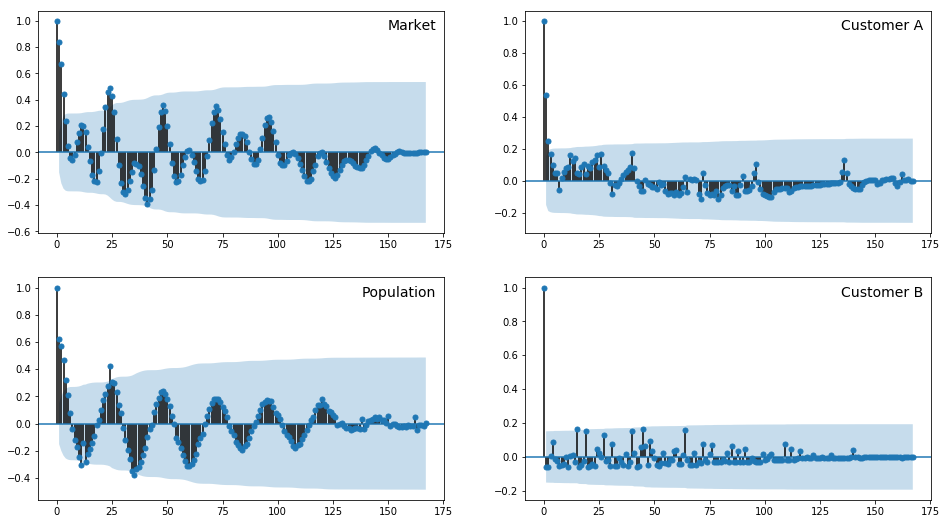
\includegraphics[width=1.0\linewidth]{img/demand_7.png}
    \caption{Lag Plot showing the correlation of the population usage data in relation to the time lag}
    \label{fig:demandtimelag}
\end{figure}

The analysis additionally showed large differences in the demand profile of different customers. Some consume several thousand
\ac{kWh} per time slot while most normal consumers only use small amounts. However, this is not directly
translatable into tariff market actions because some customers just represent the population model that simulates many
thousand individuals. Usage is not reported as individuals but rather as a sum. These models may create contracts with a
number of brokers, breaking down the demand into several small transactions spread across tariffs.

This section describes the development of the demand estimator using neural networks. It also describes the issues
observed when designing this model, which are common issues when designing prediction models using neural networks.

\subsubsection{Preprocessing existing data}
\label{sub:preprocessing}

%TODO decide if splitting to clearly DEMAND / WHOLESALE impl

To learn from the large amount of data already available from previous simulations, parsing the state files provided by
the simulation is a reasonable approach to boost the ability of several parts of the agent to learn faster. It is
especially ideal for the predictor, as it is a supervised problem.

A first approach was to manually parse these files and reconstruct the server state in python.
While this was successful for the demand component, the powertac-tools repository was discovered to hold similar tools
based on a combination of python and java components. This repository allows the creation of customer production and
consumption information in a comma separated file format. Each tool creates a csv file with a specific focus instead of
parsing all information in one central loop. The initial approach to parse the files was thus scrapped
and replaced with this prebuilt variant that makes use of the powertac-server source code.

While the current demand prediction is solely based on historical demand, this can easily be extended (as it has been in
the python only approach previously mentioned) with weather data, time information and up-to-date tariff
information\footnote{All preprocessing code has been deleted in commit
    \href{https://github.com/pascalwhoop/broker-python/commit/c54ee7c05585d15462f40e2be6850343e8aea27a}{c54ee7c} in the
broker-python repository.}.



%The general architecture of the agent follows the idea of a core \emph{environment} module that holds all relevant data
%for a game. Tariffs, rates, customers, transactions and other data is stored in this module. Since the state files are
%based on events (they hold constructor parameters and method call parameters of previous server instances), these events
%need to be applied to the environment. To learn from these events, most modern frameworks require a training
%data-set and a label data-set. Therefore these events are first applied to the environment and at each time slot,
%relevant training samples are extracted. Therefore the overall structure of the translation from state files to training
%data is as follows:

%\begin{enumerate}
%    \item Iterate over all local state files
%    \item Iterate over lines in state file
%    \item Apply line to
%        current environment state
%    \item At each time slot, extract relevant samples
%    \item Store training data in separate local
%        %TODO separate vs online/streaming structured approach
%files \end{enumerate}
%
%The code linked to the process described above is part of the \texttt{util.state\_extractor} and
%\texttt{model.environment} modules. The tests in the \texttt{tests} module document the functionality.
%
%After the translation, the data is usually structured in a multi-dimensional array which can be read by numpy and
%processed with Keras. First, some preprocessing can be applied with scikit-learn to analyze the structure of the data as
%well as ensure the values that are fed to the neural network don't negatively impact the learning progress. The overall
%approach follows the recommendations of \citep{Goodfellow-et-al-2016}.

\subsubsection{Model design phase}%
\label{sub:model_design}



From a dependency perspective, this component has no dependencies onto the other learning components and can easily be
trained using historical data. It is a supervised learning algorithm, matching known information in time slot
$t-n$ to a prediction for the expected energy usage at time slot $t$. Because there are several games on record, the
historical realized usages are the labels for the supervised learning problem. Known information includes: weather
forecasts, historical usages, time, tariff and customer metadata. A simplest approach and thus a baseline to
measure against is to predict the customer to consume the same amount as in the previous time slot. All demand
prediction loss is measured in mean squared error.

%A random prediction based on a neural network being fed random data usually
%levels out at 300 to 400. This gives a goal range (below -24h prediction) as well as a pattern to avoid which
%basically equals not learning anything.
Several standard architectures were tried. However, none significantly outperformed a simple heuristic approach such as
guessing the demand to be equivalent to that of 24 hours ago. A later analysis\footnote{see Jupyter notebooks for Demand
Estimator}
revealed why this occurs. The neural networks architectures are having trouble handling both very large and very small
customer patterns. When training a neural network for each customer individually, the performance is much higher. This
intuitively leads to the idea that creating a model for each customer may lead to a performance boost. This 
creates a range of other complications. Most frameworks are written based on the assumption that one neural network is
trained per machine. Most neural networks are only limited by the amount of available hardware and data. Having some
200+ neural networks learning from data and predicting in parallel, all in less than five seconds per time slot is hard
to achieve on conventional hardware. A test run showed that the system can only
process one customer every three seconds. It was therefore necessary to either add significant amount of processing
power to the broker or somehow get one model to predict all kinds of customer classes with decent precision. One
improvement was the creation of a separate preprocessing scaler for each customer. While the previous approach used one
\texttt{MinMaxScaler} that scales all values between two limits, usually 0 and 1, the second approach included the
creation of a scaler for each customer, to allow for an individual scaling across customers. The difference is visualized
in Figure~\ref{fig:imgfrosty} and it allows for clearer signals to be received by the network.
%TODO cont in Figure~\ref{fig:demand_baseline}.


\begin{figure}[]
    \centering
    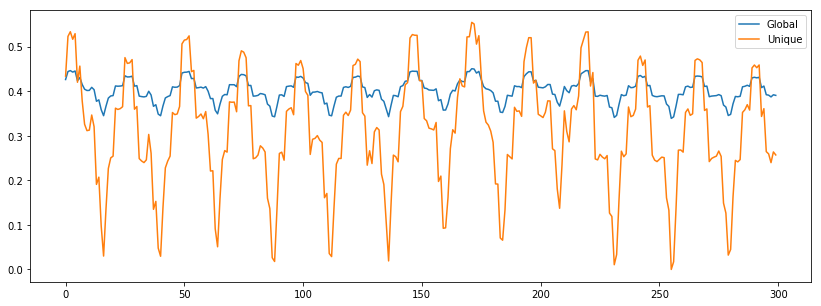
\includegraphics[width=1.0\linewidth]{img/frosty_scaled.png}
    \caption{Comparison of scaled data with unique scaler (yellow) or global scaler (blue)}
    \label{fig:imgfrosty}
\end{figure}

Ultimately, the predictor model that seemed most successful in terms of average error and robustness against repetitive
training on various types of usage patterns was a dense vanilla feed-forward neural network with
\texttt{168,100,50,24} units. The optimizer uses stochastic gradient descent (LR=0.01) and the layers mostly use
\ac{ReLu} activation functions except for the last one which is a linear function. To overcome the problem of
catastrophic forgetting, a common phenomenon observed when networks were trained on several tasks in sequence
\citep{french1999catastrophic}, all input data is shuffled instead of processed in sequence per customer. While this
does not keep the network from forgetting, it makes it forget learned knowledge about patterns uniformly, replacing the
previous weights with newly learned weights from newly observed patterns uniformly. Results for this predictor are shown
in Figure~\ref{fig:imgcombined_model}, a comparison with the baseline and more examples of various customer types of
-24h are given in the appendix. It is visible from the figure that the model has learned to predict regular
spikes. It doesn't seem to understand that there is a natural maximum to the usage pattern, which is understandable for
a continuous model. It also doesn't capture the reduced usage on every 7th day as can be seen via the flat hump
in the brown realized curve. An \ac{LSTM} model is usually considered to be successful with these kinds of problems but
my experiments did not succeed. A comparison between the baseline, a vanilla feed-forward and an \ac{LSTM} model is
shown in Figure~\ref{fig:baseline_dense}

\begin{figure}[b]
    \centering
    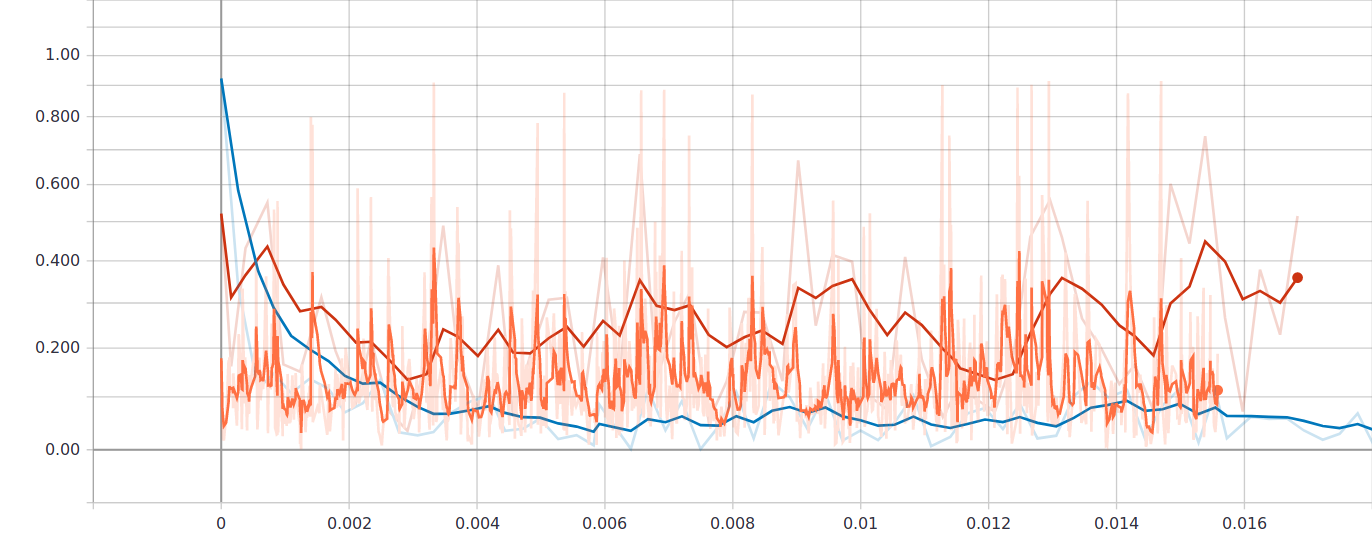
\includegraphics[width=1.0\linewidth]{img/demand_baselines_2.png}
    \caption{Demand baselines and models, -24h baseline: orange, lstm: red, dense: blue}
    \label{fig:baseline_dense}
\end{figure}


The timing of this unified model is also acceptable with 3 to 4 ms per 24h forecast required, adding up to a 800 ms
delay for predicting 200 customers, which would almost cover the entire games customer base.

\begin{figure}
    \centering
    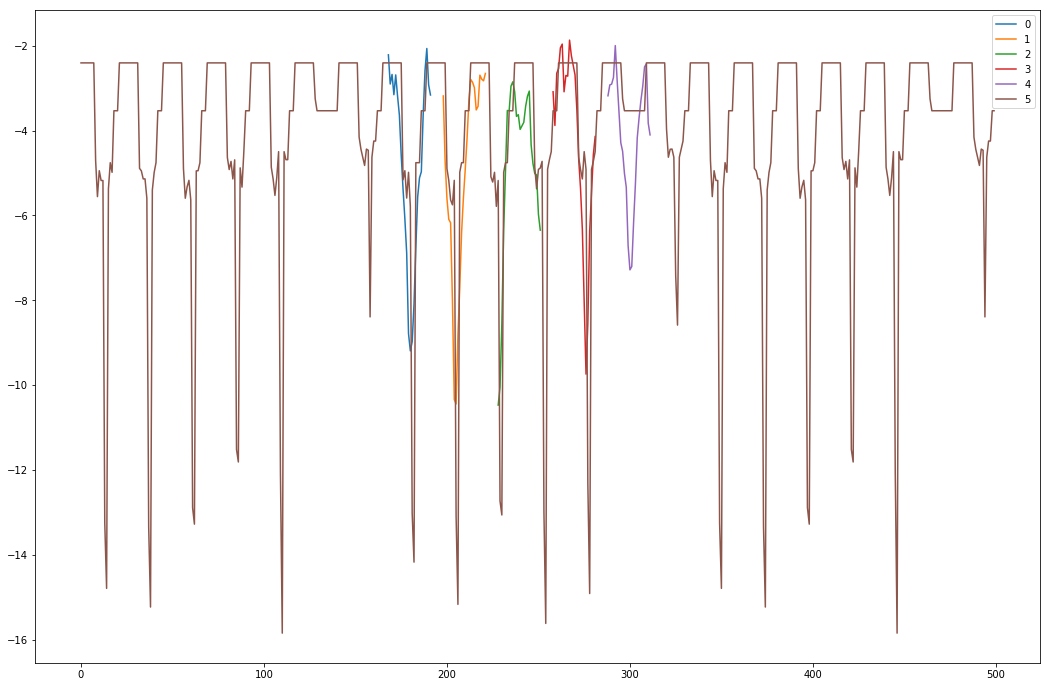
\includegraphics[width=1.0\linewidth]{img/pred1.png}
    \caption{Plotting of forecasts and realized usage}
    \label{fig:imgcombined_model}
\end{figure}



%If the customer models change across games (e.g.\ if a customer suddenly uses 10x the energy on rainy days), the learning
%model will have to learn to adapt to this change. This can be achieved by letting the model both learn from historical
%data initially (i.e.\ form the state files) and also let it learn online during the competition, based on the new
%customer models.
%
%To train a model that predicts the demand amounts of customers under various conditions, a dataset of features and
%labels needs to be created. Because the model may also learn during the course of a running competition, a generator
%based structure should be preferred. This means that a generator exists that creates $x, y$ pairs for the model to train
%on, instead of creating a large batch of learning data ahead of the learning processing, which is otherwise a common
%practice. Whenever a round completes and new information is available, the demand estimator is asked to estimate the
%demand for all customers subscribed to the tariffs of the broker for the next 24 time slots. These estimations are then
%saved (i.e.\ they replace any previous estimations) and the wholesale component as well as other components can act on
%this newly created estimations.

%According to the simulation specification, the customer models generate their demand pattern based on their internal
%structure, broker factors and game factors \citep[]{ketter2018powertac}. The preprocessing pipeline of the generator therefore generates
%feature-label pairs that include: Customer, tariff, weather, time and demand information. The realized demand is the
%label while all other components are part of the features that are used to train the model. The intuitive model class
%for demand patterns prediction are \ac{RNN} due to the sequential nature of the problem \citep[]{EvalGRU2014}. However,
%as will be shown later, the implementation of relatively shallow dense classic neural network also results in decent results.

\begin{figure}[h]
    %TODO export new variant in drawio
    \centering
    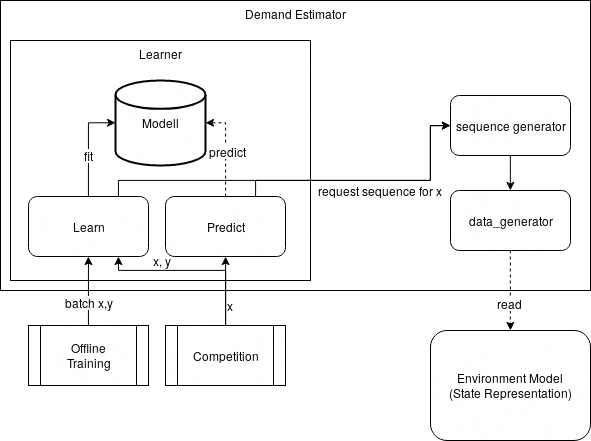
\includegraphics[width=1.0\linewidth]{img/UsageEstimator.png}
    \caption{Demand Estimator structure}
    \label{fig:DemandEstimator}
\end{figure}

\subsubsection{Integrating the model into the python broker}%
\label{sub:integrating_the_model_into_the_python_broker}

Once the general concept of the learning model was decent, the model had to be integrated into the broker framework and
a surrounding architecture had to be built to allow this network to learn and predict live in a game setting.
The overall structure of the demand estimator component is shown in Figure~\ref{fig:DemandEstimator}. The model can be
both trained offline based on the state files and online during the competition. This is possible because in both
situations, the environment model of the agent is a continuous representation of the agents knowledge about the world.
In fact, during the state file parsing, the environment may even hold information that the agent usually cannot observe
in a competition environment. This is also the case for the demand learning, as the state files hold the demand
realizations of all customers while the server  only transmits the usage realizations of the
customers that are subscribed to the agents tariffs during the competition. Regardless, this does not affect the ability to learn from the
customers usage patterns in either setting.

During a competition, the agent may learn from the realized usage of
customers after each time slot is completed. The server transmits TariffTransaction objects for each time slot that hold
the energy usage of the subscribed subset of all customers of each customer model. To avoid mismatching predictions,
these subset usages are scaled up to the whole population count for the prediction step. Afterwards, the values are
scaled back down to the actual subscription partition of the customer model.

Because the process of learning from newly observed data may require some resources, it is advantageous to
first perform the prediction of the subscribed customers demands for the current time slot to pass this information to
the wholesale component before training the model on the received meter readings. While the broker is waiting for the
server to process a step in the game, it can perform any learning on newly received information\footnote{The component code can be
found under \url{https://github.com/pascalwhoop/broker-python/tree/master/agent_components/demand}}. A sketch of the
core loop is shown in Listing~\ref{lst:estimatorpseudo}.

\begin{listing}
    \begin{minted}[linenos,numbersep=5pt,frame=lines,framesep=2mm]{python}
handle_timeslot():
   X,Y,X_PRED = prep_data()
   if not X or Y or X_PRED:
       return
   pred = model.predict(X_PRED)
   pred = scaler.inverse_transform(pred)
   pred = correct_customer_count(pred)
   # dispatch to pubsub
   dispatcher.send(pred)
   model.fit(X,Y)
    \end{minted}
    \caption{Pseudocode for estimator loop}
    \label{lst:estimatorpseudo}
\end{listing}



%TODO write final model structure and plot against intuitive -24h baselines

\subsection{Wholesale market}
\label{sec:wholesale_market}

To approach the wholesale trading problem, a subset of the definition of the trading problem developed by
\citet{tactexurieli2016mdp} was assumed. More specifically, the agent only concerns itself with the activities in the
wholesale market and does not act or evaluate tariff market or balancing market activities. This is due to the
separation of concern approach described earlier. Therefore, it is a \ac{MDP} that can be solved with \ac{RL} techniques.
The goal was the ability to apply current and future deep \ac{RL} implementations to the \ac{PowerTAC} problem set. For this,
many of the previously described implementations were necessary. Now that a Python based broker is possible, the application
of \ac{PPO}, \ac{DQN} and other modern \ac{RL} agent implementations seems reasonable. All required messages can be
subscribed to via the publish-subscribe pattern. What is missing are the following components which are explained in
detail in this section:

\begin{itemize}
    \itemsep0em
    \item A mapping from the 24 parallel environments to a single \ac{MDP} environment
    \item A correction of the common paradigm where the agent is in control of the program flow
    \item A solution to the problem that one agent is supposed to be in control of and learn from several
        environments in parallel
    \item A way to learn quickly from offline data
    \item Suitable reward functions
    \item Input preprocessing
    \item An initial implementation of a \ac{RL} agent using modern deep neural network frameworks
\end{itemize}


\subsubsection{\acs{MDP} design comparison}%
\label{ssub:mdp_design_comparison}

There are two possible ways of modeling the \ac{MDP}: per time slot or per game. Per time slot is aligned to the
definition by \citet{tactexurieli2016mdp}. Per game considers each game a unified \ac{MDP} where the agent acts in all
time slots and has an action space of 48 values per time slot.

%Termination occurs when there are no further trading opportunities for a time slot and the \ac{DU} applies the final
%balancing fee to the time slot. Brokers that have predicted their usage precisely and traded matching amounts of energy
%in the wholesale market require less balancing than those that either suffer bad forecasting or are not capable to place
%orders successfully before the trading is closed. The \ac{RL} reward function may be composed in different ways but a
%very intuitive approach is to use the profit achieved by the broker for the given time slot. Because this reward design
%suffers strong noise from the market price fluctuations, different reward functions may be preferred as discussed later.

Both approaches have advantages and disadvantages. The former creates short, fixed-length episodes that more closely
match the concepts of contemporary \ac{RL} problems such as the locomotion examples described in
Section~\ref{sub:deep_learning_in_reinforcement_settings}. However, because \ac{PowerTAC} allows for trading up to 24 hours into the future, 24
environments would have to be stepped in parallel. Approaches for parallel asynchronous stepping of multiple
environments with a neural network based policy function approximator exist \citep{mnih2016asynchronous,hafner2017agents}
but they require more complex architectures that update a central policy function based on experiences from all environments.
The latter avoids this, allowing a fairly simple off-the-shelf algorithm to be applied to the problem. Issues appear
with the compatibility to the action spaces this agent requires as well as the increased signal noise. Common algorithms
such as \ac{DQN}, \ac{SARSA} or \ac{A3C} are not easily applied to such large action spaces. They are written to be
applied to discrete action spaces \citep{baselines}. \ac{PowerTAC} trading is in its purest form a continuous action
space, allowing the agent to define both amount and price for a target time slot. Furthermore, the agent would observe
information for 24 open time slots in parallel and generate 24 largely independent trading decisions. The network would
have to learn to match each input block to an output action, as the input for time slot 370 has little effect on the
action that should be taken in time slot 380. In a separated \ac{MDP}, each environment observation would only hold the
data needed for the specific time slot rather than information about earlier and later slots.

\subsubsection{\acs{MDP} implementation}%
\label{sub:mdp_design_and_implementation}

After considering the entire simulation as a single \ac{MDP}
\footnote{\url{https://github.com/pascalwhoop/broker-python/blob/5876c2d5044102d3fbff4bde48b5febfdb15a84f/agent_components/wholesale/mdp.py}}
but not seeing any successful learning, the separated approach was chosen.

To separate the messaging from the \ac{MDP} logic, as well as to separate the 24 environments parallelism complexity
from the individual \ac{MDP}, several layers of abstraction were introduced. First, all relevant messages are
subscribed to in the \texttt{WholesaleEnvironmentManager} using the publish subscribe pattern. Individual messages are
then passed along to the corresponding active \ac{MDP} and new environments are created for every newly activated
time slot. Therefore, the \texttt{WholesaleEnvironmentManager} abstracts the multiplicity complexity from the individual
\texttt{PowerTacEnv}.

The individual \ac{MDP} environments receive a reference to the \ac{RL} agent during creation so that they can pass
their observations to it and request actions as well as trigger learning cycles on received rewards. This means that
each individual \ac{MDP} is not aware of other instances. While reducing complexity, it also hinders the ability of
the learning agent to consider its impact of trading in time slot $t$ on any future time slots. The message flow is
depicted in Figure~\ref{fig:ws_msg_flow}.

% doesn't fit on the page without cutting off the right side...
%\begin{listing}
%    \begin{minted}[linenos,numbersep=5pt,frame=lines,framesep=2mm]{python}
    %def subscribe(self):
    %  """Subscribe to any newly incoming messages from the server"""
    %  disp.connect(self.handle_market_transaction, signal=PB_MARKET_TRANSACTION)
    %  disp.connect(self.handle_timeslot_update, signal=PB_TIMESLOT_UPDATE)
    %  disp.connect(self.handle_cleared_trade, signal=PB_CLEARED_TRADE)
    %  disp.connect(self.handle_predictions, signal=COMP_USAGE_EST)
    %  disp.connect(self.handle_tariff_transaction, signal=PB_TARIFF_TRANSACTION)
    %  disp.connect(self.handle_market_bootstrap_data, signal=PB_MARKET_BOOTSTRAP_DATA)
    %    \end{minted}
%    \caption{Environment manager listening to all relevant message types}
%    \label{lst:subscribeenvmanager}
%\end{listing}


\begin{figure}[h]
    \centering
    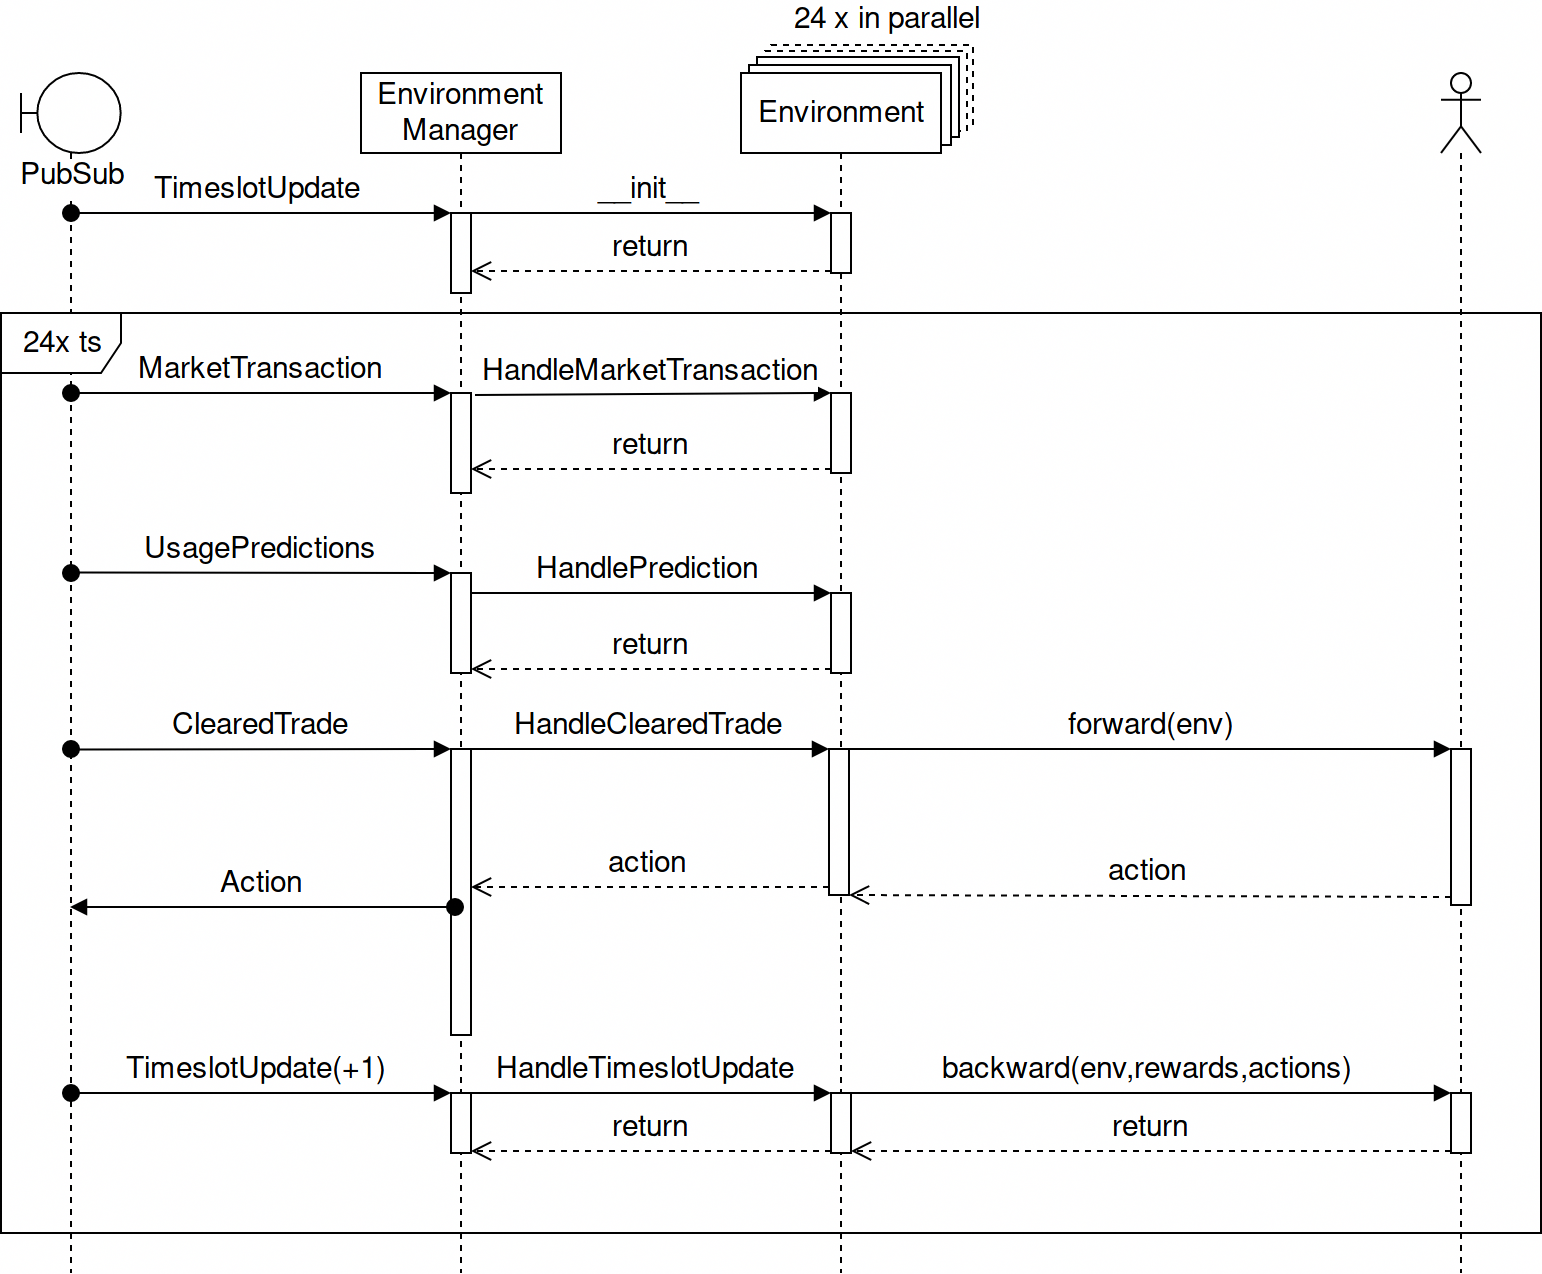
\includegraphics[width=1.0\linewidth]{img/WholesaleComponent.png}
    \caption{Wholesale component message flow}
    \label{fig:ws_msg_flow}
\end{figure}

\subsubsection{Reversal of program flow control}%
\label{sub:reversal_of_flow_control}

The environment expects the agent to expose an \ac{API} that includes two calls: \texttt{forward} and
\texttt{backward}. This pattern has been adopted from the keras-rl and Tensorforce libraries. The reason is simple:
while most libraries put the agent in control of the program flow, the \ac{PowerTAC} broker will be stepped by the
server and the \ac{RL} agent itself has no control of the flow. The forward and backward methods are
directly aligned with the keras-rl framework and easily applicable to the Tensorforce \texttt{act()} and
\texttt{atomic\_observe()} methods of their agent implementations. The abstract \texttt{PowerTacWholesaleAgent} class just defines a
few methods that need to be implemented by a developer to create a new algorithm for the wholesale trading
scenario. In this work, the \texttt{TensorforceAgent} class represents an example implementation and it holds several
configurations for a number of architectures. The \texttt{BaselineAgent} simply trades the prediction
energy amount for generous market prices. This is useful to compare performance of a learned algorithm with a very
intuitive trading scheme and to serve, as the name suggests, as a baseline.

The reversal of flow control has another benefit: while other approaches had to create specific designs to allow 
several agents to act in several environments with one \emph{main agent} to adopt those network changes, this is not
required because the environments are calling the agent. The environments are all using one agent instance to learn and
act and the environment manager is triggering the environments in sequence. \citet{mnih2016asynchronous} discuss 
benefits and drawbacks of experience replay based learning and their asynchronous parallel stepping approach which
allows on-policy learning algorithms. In the implementation, all environments first request an action and then trigger
the \texttt{backward} function that triggers the agents learning process. While this is currently not batched and
leads to a changed policy after the first update has been completed, it could be batched into
one learning policy update, enabling on-policy algorithms to be used. The problem of correlated states and
non-stationarity that was first solved by experience replay in \citep{mnih2013playing} is solved similarly to what
\citet{mnih2016asynchronous} describe, i.e.\ by having several environments updating the agent, decorrelating the
sequence of observation-action inputs.

\subsubsection{Learning from historical data}%
\label{sub:learning_from_historical_data}

Learning quickly from historical data may be facilitated for off-policy algorithms that can learn from historical
records of other agents or, if the approach introduced in
Section~\ref{ssub:offline_record_based_wholesale_environment_approximation} is applied, also for on-policy algorithms by
approximating the real environment based on the historical data.
The \texttt{LogEnvManagerAdapter.py} class allows reuse of existing algorithm implementations. It
parses historical files and sends events via the event dispatcher as if they originated from the server. This way, the
same code may be used to train online in a competition or offline from historical data. It iterates over the existing
game logs and generates both forecasts for the \ac{RL} agent as well as all necessary events that trigger the \ac{RL}
agent. The forecasts can optionally be based on the actual demand estimator or they can be the arbitrarily noisy real
values. This means that the agent can be trained with perfect predictions all the way to very bad predictions.

\subsubsection{Reward functions}%
\label{sub:reward_functions}

Well crafted reward functions are elementary for any non-trivial \ac{RL}
environment \cite[p.469ff.]{amodei2016concrete, sutton2018reinforcement}. While the Atari agents often receive their reward directly from the
game as many games include a game point counter \citep{mnih2013playing}, \ac{PowerTAC} technically simulates a
real-world energy market which means the score equals the brokers profit. Nonetheless, the profit is dependent on a number of
factors where the wholesale trading component only makes up a comparatively small part and thus it is hardly a
good choice for a reward proxy. Using the purchase prices of the energy purchased is also noisy, as it depends on the
supply and demand of the entire market. Generally, the broker attempts to trade energy at a good price which can be
defined as one that is better than those of other participants in the market. A reward function based on the relation
between the average price paid by the broker and the average price paid by the overall market hence describes
how well the agent did in comparison to the others and consequently removes the market price fluctuation noise from the
reward values.

To calculate this reward, all the purchases of the agent as well as all market clearings are averaged for a given target
time slot.

\begin{equation}
    r_{rel} = \left\{
        \begin{array}{lr}
            \bar{p_b} / \bar{p_m}, & \text{for } sum(q) \leq 0 \\
            \bar{p_m} / \bar{p_b}, & \text{for } sum(q) > 0
    \end{array}\right\}
\end{equation}

Defines the reward, where $\bar{p}$ is determined by

\begin{equation}
    \bar{p} =\frac{\sum ^{1}_{i=24} p_{i} *q_{i}}{\sum ^{1}_{i=24} q_{i}}
\end{equation}

for both the market averages and the broker averages. This encourages the agent to buy for low prices and to sell for high
prices when possible. $sum(q)$ is the net purchasing amount after the 24 trading opportunities are completed, i.e.\ it
describes if
the broker ended up with a positive or negative net flow of energy in the wholesale market. This reward function has one
immediate drawback: it can only be calculated once the market for the target time slot is closed. Therefore, the agent 
doesn't get any feedback during any step except the terminal state.

While \ac{RL} research has stated sparse reward as a core part of \ac{RL}, many of the recent algorithms do
not deal well with such sparse rewards. Experience replay partially works so well in the Atari domain due to the dense
reward structure of the domain, allowing randomly selected transitions from the replay buffer to hold information for
the agent at any stage of the learning phase \citep{schaul2015prioritized}.
To improve information density in the powertac environment it may be beneficial to provide further feedback to the
trader agent. The wholesale trader gets a prediction for a target time slot at every of the 24 slots prior to the
target. These predictions come from a specialized demand predictor component and the wholesale trader would do well 
trusting the prediction to some degree. A good wholesale trader mostly does well in buying sufficient energy for the target
time slot to ensure its portfolio is balanced as the forced \ac{DU} balancing is usually more costly than buying energy
ahead of time. The reward function may hence be extended by a term that punishes large
deviations from the predicted required amounts.


\begin{equation}
    r_{\text{pred}} = - | \text{action} - (\text{purchased before} + \text{prediction}) | * \frac{\text{step}}{24}
\end{equation}

Here, the divergence of the action and the required energy is multiplied with a factor that describes the \emph{urgency}
of the balancing. The closer the target time slot becomes, the more urgent is a balanced portfolio.

The final reward is now a combination of those two reward terms. The first reward function $r_{rel}$ puts emphasis on purchasing
energy for a good price, no matter how the agent purchases it (e.g.\ by buying early and selling later for higher
prices) while the second puts emphasis on purchasing energy in accordance with the portfolio predictions.
\begin{equation}
    r_{comb} = \left\{
        \begin{array}{lr}
            r_{rel} & \text{if TS} = 24 \\
            r_{pred} & \text{else}
        \end{array}
    \right\}
\end{equation}

This function has another benefit that became obvious during the experiments: if the offline trading approximation
assumes the broker has no influence on the market price and if the reward function does not punish large orders, the
broker quickly starts ordering energy several orders of magnitude larger than the overall market size. It learned that
there is virtually free leverage which can be used to profit from market price fluctuations. By adding the
prediction as a limiting factor, the agent is encouraged to not try and trade absurdly large amounts of energy but to
simply trade amounts that match its demand. This flaw is due to the way the offline data based environment approximation
determines the closing prices which don't depend on the agents orders. It is different from the real wholesale market
where the price is influenced by any market participant.

Other reward functions are present in the \texttt{reward\_functions.py} file such as an automatically adjusting one that
at first strongly punishes balancing and disregards the price but shifts towards the price based reward once the
balancing amounts are reduced. Generally, more work is required to construct a better reward function.
Reward functions are difficult to design, because systems tend to overfit on the reward function in a way that the
results do not intuitively make sense but optimize towards the slightly misdefined reward function
\citep{amodei2016concrete}.

\subsubsection{Input preprocessing}%
\label{sub:input_preprocessing}

The inputs can be preprocessed in a number of ways. Because each \ac{RL} agent implementation may be interested in a
different subset of the environment to base its decision on, the agent implementation gets passed the entire environment
object.
My agent implementation (\texttt{Tensorforce.py})
expects the previous 168 time slot price averages, all prior forecasts as well as all prior purchases for the
target time slot. In a first attempt, these 216 values were flattened into a one-dimensional input array and fed
to the agent as an observation. Without any preprocessing, this implementation was not able to converge towards a good
reward indicating learning progress. Preprocessing was introduced based on the already described MinMaxScaler,
scaling all prices and prediction amounts to a fixed scale. To permit easily configuring the agent with a variety of
preprocessing functions, a CLI parameter was introduced. The parameter value has to correspond to a function in the
\texttt{agent\_components/wholesale/learning/preprocessor.py} file.

\subsubsection{Tensorforce agent}%
\label{sub:tensorforce_agent}

Now to pull the components together, the agent receives \texttt{forward} and \texttt{backward} calls from
the environment, returns actions and learns when passed the required information. The development of \ac{RL} agents
includes a lot of trial and error which led to the creation of another \ac{CLI} endpoint called \texttt{wholesale}. The
\ac{CLI} allows the custom selection of the reward function, action type, network structure, agent type and tagging the
trial with custom strings. It starts an instance of the \texttt{LogEnvManagerAdapter} which runs through recorded
games and simulates the necessary events. To run several trials, a helper tool that automatically generates
these CLI calls was created that runs all variations of them in sequence. In total, dozens of offline simulation approximations were
run during the development and a set of 72 configurations were run as a final analysis with a variety of
hyperparameters. Each run included 5 simulated games which result in roughly 200.000 learning steps and the average
reward of the last game is considered the final performance of that run. Table~\ref{tab:trading} summarizes all trials
executed.

\begin{table}[]
    \caption{Wholesale offline trading results overview  for various hyperparameters}
    \label{tab:trading}

    \resizebox{\textwidth}{0.48\textheight}{
        \begin{tabular}{l|l|l|l|l|l}
            \textbf{Network} &       \textbf{r\_type} &       \textbf{Preprocessing} &   \textbf{Action\_T} & \textbf{agent\_type} & \textbf{average r after 5 games} \\ \hline
            vnn32x2          &       $r_{rel}$        &       simple                 &   continuous         & vpg                  & -39        \\
            vnn32x2          &       $r_{rel}$        &       simplenorm             &   continuous         & vpg                  & -39        \\
            bn\_vnn32x2      &       $r_{rel}$        &       simplenorm             &   continuous         & vpg                  & -39        \\
            bn\_vnn32x2      &       $r_{rel}$        &       simple                 &   discrete           & vpg                  & -46        \\
            vnn32x2          &       $r_{rel}$        &       simplenorm             &   twoarmedbandit     & dqn                  & -83        \\
            bn\_vnn32x2      &       $r_{rel}$        &       simplenorm             &   continuous         & random               & -110       \\
            vnn32x2          &       $r_{rel}$        &       simplenorm             &   discrete           & dqn                  & -120       \\
            bn\_vnn32x2      &       $r_{rel}$        &       simple                 &   continuous         & dqn                  & -157       \\
            vnn32x2          &       $r_{rel}$        &       simple                 &   twoarmedbandit     & vpg                  & -225       \\
            bn\_vnn32x2      &       $r_{rel}$        &       simplenorm             &   discrete           & dqn                  & -297       \\
            bn\_vnn32x2      &       $r_{rel}$        &       simple                 &   discrete           & random               & -445       \\
            vnn32x2          &       $r_{rel}$        &       simplenorm             &   continuous         & random               & -474       \\
            vnn32x2          &       $r_{rel}$        &       simple                 &   twoarmedbandit     & random               & -508       \\
            bn\_vnn32x2      &       $r_{rel}$        &       simplenorm             &   continuous         & dqn                  & -673       \\
            bn\_vnn32x2      &       $r_{rel}$        &       simple                 &   continuous         & random               & -840       \\
            bn\_vnn32x2      &       $r_{rel}$        &       simple                 &   twoarmedbandit     & random               & -899       \\
            bn\_vnn32x2      &       $r_{rel}$        &       simplenorm             &   twoarmedbandit     & vpg                  & -1077      \\
            bn\_vnn32x2      &       $r_{comb}$       &       simplenorm             &   discrete           & vpg                  & -1297      \\
            vnn32x2          &       $r_{comb}$       &       simple                 &   discrete           & vpg                  & -1959      \\
            bn\_vnn32x2      &       $r_{rel}$        &       simple                 &   twoarmedbandit     & vpg                  & -2289      \\
            bn\_vnn32x2      &       $r_{comb}$       &       simple                 &   continuous         & vpg                  & -2396      \\
            bn\_vnn32x2      &       $r_{comb}$       &       simplenorm             &   discrete           & dqn                  & -3229      \\
            vnn32x2          &       $r_{comb}$       &       simplenorm             &   discrete           & vpg                  & -3434      \\
            vnn32x2          &       $r_{comb}$       &       simplenorm             &   discrete           & dqn                  & -3836      \\
            vnn32x2          &       $r_{rel}$        &       simple                 &   continuous         & dqn                  & -4567      \\
            bn\_vnn32x2      &       $r_{rel}$        &       simple                 &   discrete           & dqn                  & -5460      \\
            vnn32x2          &       $r_{comb}$       &       simplenorm             &   discrete           & random               & -5560      \\
            bn\_vnn32x2      &       $r_{rel}$        &       simple                 &   continuous         & vpg                  & -6078      \\
            bn\_vnn32x2      &       $r_{rel}$        &       simple                 &   twoarmedbandit     & dqn                  & -6809      \\
            bn\_vnn32x2      &       $r_{comb}$       &       simple                 &   continuous         & random               & -7791      \\
            bn\_vnn32x2      &       $r_{comb}$       &       simple                 &   discrete           & random               & -7907      \\
            vnn32x2          &       $r_{rel}$        &       simple                 &   continuous         & random               & -8694      \\
            vnn32x2          &       $r_{comb}$       &       simple                 &   discrete           & dqn                  & -9376      \\
            bn\_vnn32x2      &       $r_{comb}$       &       simple                 &   discrete           & vpg                  & -11102     \\
            bn\_vnn32x2      &       $r_{comb}$       &       simple                 &   discrete           & dqn                  & -12175     \\
            vnn32x2          &       $r_{comb}$       &       simple                 &   continuous         & dqn                  & -12531     \\
            vnn32x2          &       $r_{comb}$       &       simple                 &   discrete           & random               & -13147     \\
            bn\_vnn32x2      &       $r_{comb}$       &       simplenorm             &   discrete           & random               & -13511     \\
            vnn32x2          &       $r_{comb}$       &       simple                 &   continuous         & random               & -25061     \\
            vnn32x2          &       $r_{rel}$        &       simplenorm             &   continuous         & dqn                  & -25762     \\
            vnn32x2          &       $r_{comb}$       &       simplenorm             &   continuous         & dqn                  & -27761     \\
            bn\_vnn32x2      &       $r_{comb}$       &       simplenorm             &   continuous         & random               & -35308     \\
            vnn32x2          &       $r_{comb}$       &       simplenorm             &   continuous         & random               & -36619     \\
            bn\_vnn32x2      &       $r_{comb}$       &       simple                 &   continuous         & dqn                  & -44376     \\
            bn\_vnn32x2      &       $r_{comb}$       &       simplenorm             &   continuous         & dqn                  & -52547     \\
            vnn32x2          &       $r_{rel}$        &       simple                 &   twoarmedbandit     & dqn                  & -60246     \\
            vnn32x2          &       $r_{rel}$        &       simplenorm             &   discrete           & random               & -60473     \\
            bn\_vnn32x2      &       $r_{comb}$       &       simplenorm             &   continuous         & vpg                  & -95084     \\
            vnn32x2          &       $r_{rel}$        &       simple                 &   discrete           & dqn                  & -127978    \\
            bn\_vnn32x2      &       $r_{rel}$        &       simplenorm             &   twoarmedbandit     & dqn                  & -276400    \\
            vnn32x2          &       $r_{comb}$       &       simplenorm             &   twoarmedbandit     & vpg                  & -296235    \\
            bn\_vnn32x2      &       $r_{comb}$       &       simple                 &   twoarmedbandit     & dqn                  & -299472    \\
            vnn32x2          &       $r_{rel}$        &       simple                 &   discrete           & random               & -394223    \\
            bn\_vnn32x2      &       $r_{comb}$       &       simplenorm             &   twoarmedbandit     & random               & -543207    \\
            bn\_vnn32x2      &       $r_{rel}$        &       simplenorm             &   twoarmedbandit     & random               & -592135    \\
            vnn32x2          &       $r_{rel}$        &       simplenorm             &   discrete           & vpg                  & -722341    \\
            bn\_vnn32x2      &       $r_{comb}$       &       simple                 &   twoarmedbandit     & vpg                  & -939824    \\
            vnn32x2          &       $r_{rel}$        &       simple                 &   discrete           & vpg                  & -1035320   \\
            bn\_vnn32x2      &       $r_{comb}$       &       simple                 &   twoarmedbandit     & random               & -1060802   \\
            bn\_vnn32x2      &       $r_{rel}$        &       simplenorm             &   discrete           & random               & -1083496   \\
            bn\_vnn32x2      &       $r_{comb}$       &       simplenorm             &   twoarmedbandit     & vpg                  & -1188154   \\
            vnn32x2          &       $r_{rel}$        &       simplenorm             &   twoarmedbandit     & random               & -1311061   \\
            vnn32x2          &       $r_{comb}$       &       simplenorm             &   twoarmedbandit     & dqn                  & -1608152   \\
            bn\_vnn32x2      &       $r_{rel}$        &       simplenorm             &   discrete           & vpg                  & -1644698   \\
            vnn32x2          &       $r_{comb}$       &       simple                 &   twoarmedbandit     & dqn                  & -2018251   \\
            vnn32x2          &       $r_{comb}$       &       simplenorm             &   twoarmedbandit     & random               & -3127925   \\
            vnn32x2          &       $r_{rel}$        &       simplenorm             &   twoarmedbandit     & vpg                  & -4188259   \\
            bn\_vnn32x2      &       $r_{comb}$       &       simplenorm             &   twoarmedbandit     & dqn                  & -43697734  \\
            vnn32x2          &       $r_{comb}$       &       simple                 &   twoarmedbandit     & vpg                  & -129692147 \\
            vnn32x2          &       $r_{comb}$       &       simple                 &   twoarmedbandit     & random               & -351135515 \\
            vnn32x2          &       $r_{comb}$       &       simple                 &   continuous         & vpg                  & nan        \\
            vnn32x2          &       $r_{comb}$       &       simplenorm             &   continuous         & vpg                  & nan        \\

        \end{tabular}
    }
\end{table}
The reward values shown in the table were received by multiplying the results of the original reward functions by 1000
to improve signal strength. The forecasting error was set at 2\% per time slot, the network configurations can be seen in
the \texttt{broker-python} repository\footnote{All trials were recorded using tensorboard and are included in the
attached DVD}.
As a frame of reference, the benchmark agent, which always orders exactly what is forecast at every time step and offers
very generous prices, achieves an average reward of 63 with a 2\% forecasting error per time slot and an average reward
of 1500 with a 0\% forecasting error.

Unfortunately, none of the trials led to a typical asymptotic growth of the reward towards a saturation limit. Most
trials lead to a fairly stable, albeit not improving reward range. Some trials caused negatively exploding rewards.
It is also not clearly visible what caused the wide range of rewards. One hypothesis is that the reward functions tried
were not describing the problem appropriately enough for the agent to make good decisions. The reward in the
\ac{PowerTAC} setting differs significantly from the reward functions in other research as it doesn't have a "way
forward". Atari game rewards are directly taken from the games high scores and the Mujoco based locomotion rewards are
describing the distance traveled \citep{heess2017emergence}. The wholesale trading reward described above, in contrast, offers no
such \emph{progressing} forward. The actions of the agent, depending on the action type configured, allow for "easy" highly
negative rewards but to achieve a good positive reward, the agent needs to find the right chain of trades that balances
the portfolio at a good price. All good actions of the first 23 steps can be ruined with a terrible trade at the end.
This doesn't apply to the formerly mentioned environments. It may also be that the agents get caught in local optima or that
some other parameter setting was overlooked by me. Another hypothesis is the lack of memory of the agent. The wholesale
trader implementations tried were all based on acyclic feed-forward networks and contained no sense of memory.
An \ac{LSTM} based approach may lead to better results, but an initial trial did not lead to an immediate improvement.

In summary, a learning neural network based algorithm that showed any significant level of
competency in the wholesale trading environment has not been achieved. Several reward function schemes, implementations
and hyperparameters have been tried but further investigation is required to determine why the performance of the agent
variants is as unsatisfying as it is.

%\begin{figure}
%\centering
%\begin{subfigure}{.5\textwidth}
%  \centering
%  \includegraphics[width=.8\linewidth]{src/}
%  \caption{A subfigure}
%  \label{fig:sub1}
%\end{subfigure}%
%\begin{subfigure}{.5\textwidth}
%  \centering
%  \includegraphics[width=.8\linewidth]{image1}
%  \caption{A subfigure}
%  \label{fig:sub2}
%\end{subfigure}
%\caption{A figure with two subfigures}
%\label{fig:test}
%\end{figure}




%Using \ac{MDP}
%
%\ac{MDP} is actually with infinite states but for analytical concept, its irrelevant. Important is: Continuous states,
%continuous actions (with some rounding to nearest .02)
%
%Bellman equation not applicable to continuous spaces. But it is also unique because its a directed acyclic graph (the
%state transition graph) 1, 2, 3, 4, ... 24
%
%theoretically it's a nonstationary \ac{MDP} because it's limited to 24 state transitions before termination (t-0)
%
%DQN --> evaluate the value of a s,a pair
%
%\ac{PPO} --> use DNN for determining what to do in a given state - maximizes "surrogate" (relation between old and new
%policy) while penalizing too extensive reward estimations (to avoid extensive updates to policy)
%
%reward is based on relative price paid in comparison to average price for given time slot.
%
%Do I implement the env interface defined by OpenAI and let the agent subcomponent imagine it's by itself? --> allows for
%A3C and many other interesting opportunities
%
%- having issues with learning the whole thing. No learning can be observed. Network output just bounces forth and back
%between -1 and 1. 'tanh' activation functions used --> explains the bouncing limits. something inside of the network
%makes it bounce so strongly.

\section{Conclusion}%
\label{sec:conclusion}

The beginning of this work described the research progress in \ac{AI} and how new neural network based
systems are able to solve problems, previously only solvable by humans. It also pointed at the incentive to
apply new techniques to important contemporary challenges, focusing on future energy markets.
\ac{PowerTAC}, a simulation of these markets was introduced as a core research initiative that explores the field by
having many researchers compete in a competitive setting and simulate profit-oriented market participants. Because
future market participants will not shy away from using \ac{AI} technologies to improve their competitiveness,
\ac{PowerTAC} contenders must be enabled to pursue these technologies to realistically represent future markets. To
enable new competition participants to quickly catch up and to generally enable the use of neural networks, the question
was raised whether imitation based \ac{RL} models may be deployable in the \ac{PowerTAC} setting.

When reviewing this work, it is obvious that the original research question was not fully answered. Several researchers
have shown that learning from other agents is possible with neural networks in \ac{RL} environments as described in
Section~\ref{sub:deep_learning_in_reinforcement_settings}. During the course of the thesis, new research by
\citet{schmitt2018kickstarting}  has also shown how significant learning performance can be improved when allowing new
agent implementations to learn from existing agents.
However, to adapt the \ac{PowerTAC} environment to a state where these research results can be applied required large
amounts of software engineering work. Many of these intermediate steps are of value in themselves as they may lay the
groundwork for future research in this intersection of two interesting domains. The artifacts created in the course of
this work allow future research to apply these exciting \ac{RL} agent technologies and transfer learning
models to energy market simulation research.

The \ac{gRPC} message adapter that bridges the gap between \ac{PowerTAC} and current \ac{RL} model technologies offers
significant performance improvements, reducing the over-the-wire message size by approximately 70\% and making serialization of objects 44x
faster.

\ac{RL} agents require many trials to converge towards a useful policy and through the historical data \ac{MDP}
approximation as well as the containerization of the \ac{PowerTAC} components, it is now easier and more efficient
to quickly train an \ac{RL} agent for several thousand steps. The container abstraction allows for an easy instantiating
of several competitions at once with different or equal configuration parameters. It also allows for easy portability of
competing brokers, allowing \ac{PowerTAC} to adhere to the current best practices for reproducible research \citep{boettiger2015introduction}.

Participants can add a number of technologies to their docker image as well as binary files such as neural network weights and
configurations. This allows the entire competition to expand beyond the realms of Java without placing a burden on other
teams to manage not only their own dependencies but also those of other brokers. It also makes it easier for the simulation
organizers to host the entire competition and all its participants on a central server cluster instead of every team connecting to
this server remotely which may avoid many of the current complexity sources such as connectivity issue handling and mandatory
time synchronization.

The required technology for counterfactual analyses, which has only been described conceptually was shown to work with
the \ac{PowerTAC} environment and an adapted \ac{PowerTAC} server allows a broker to take control of this behavior to
simulate such a counterfactual scenario.

Finally, the Python based broker implementation may be used as a base for future developers that wish to also use these
new technologies in their brokers. It serves as base implementation that may be extended and improved by others to build
better and more sophisticated brokers that make use of all the \ac{AI} technologies that are continuously created by
researchers. The ability to build a broker using TensorFlow, Keras and TensorForce technologies was shown. The
developed broker, albeit not exhibiting outstanding performance yet, trades based on decisions derived from neural network based \ac{RL}
policies and usage predictors. Clearly, a lot of work remains to be done to see if these technologies can exceed current
performances.

% FUTURE OUTLOOK / research

Future research may now look at using the neural network technologies of recent years to compete in the \ac{PowerTAC}
competition and more importantly, to develop well performing networks. The \ac{PowerTAC} competition server itself may
be adapted to incorporate the \ac{gRPC} based communication as a secondary protocol available to brokers. This would
eliminate the need for the intermediate adapter. Because neural networks are able to incorporate large input data into
their functions, all components of a broker may now make use of a larger number of input dimensions to improve their
performance. The initial demand predictor already showed promising results, completely ignoring weather, customer
metadata, market data etc.

In summary, this work offers a contribution for bringing together the socially and economically important field of
energy markets and recent developments in \ac{AI} research. Neural networks keep succeeding in a variety of
contexts and smart energy markets will not succeed without smart participants and components, carefully embedded in a
market model that incentivizes everyone to cooperate in a way that benefits the population as a whole. \ac{PowerTAC}
will help to find the right design for these markets, simulating the most advanced autonomous agents based on bleeding
edge \ac{AI} technologies.
